\documentclass[bachelor, och, diploma]{SCWeng}
% parameter-training type - one of the following values:
%    spec-specialty
% bachelor - bachelor's degree (default)
% master - master's degree program
% parameter-form of training - one of the following values:
% och - full-time (default)
% zaoch - correspondence course
% parameter-work type - one of the following values:
% referat - abstract
% coursework - coursework (default)
% diploma - thesis
% practice-practice report
% nir-research report
%    autoref    - abstract of the final thesis
% assignment-assignment for the final qualification work
% review - manager's review
% critique - review of the final work
% parameter - enable font
% times-enable the Times New Roman font (if installed)
% disabled by default
\usepackage[T2A]{fontenc}
\usepackage[cp1251]{inputenc}
\usepackage{graphicx}
\usepackage{tempora}
\usepackage{cmap}

\usepackage[sort,compress]{cite}
\usepackage{amsmath}
\usepackage{amssymb}
\usepackage{amsthm}
\usepackage{fancyvrb}
\usepackage{longtable}
\usepackage{minted}
\usepackage{array}
\usepackage[english,russian]{babel}


\usepackage[colorlinks=true]{hyperref}
\usepackage{pgfplots}
\pgfplotsset{compat=newest}% <-- moves axis labels near ticklabels (respects tick label widths)
\usepackage{listings}
\usepackage{color}
\usepackage{subfigure}

\definecolor{dkgreen}{rgb}{0,0.6,0}
\definecolor{gray}{rgb}{0.5,0.5,0.5}
\definecolor{mauve}{rgb}{0.58,0,0.82}

\setcounter{tocdepth}{4} 
\setcounter{secnumdepth}{4}


\newcommand{\eqdef}{\stackrel {\rm def}{=}}
\newcommand{\No}{\textnumero}
\newtheorem{lem}{�����}
\setminted{style=bw,
	linenos=true,
	breaklines=true,
	numbersep=5pt,
	tabsize=2,
	fontsize=\small,
	bgcolor=white}
\setmintedinline{style=bw,
	bgcolor=white,
	fontsize=\normalsize
	}	
\pgfplotsset{every axis legend/.append style={at={(0.6,1)},anchor=south west}}
%\pgfplotsset{every axis title/.style={at={(0.5,1)},above,yshift=6pt}}
\begin{document}

% Department (in the genitive case)
\chair{mathematical cybernetics and computer science}

% Work topic
\title{Study of the friendship index of nodes in growing networks based on models with preferential attachment}

% Exchange Rate
\course{4}

% Group
\group{411}

% Faculty (in the genitive case) (by default, "faculty of books")
%\department{KNiIT faculty}

% Specialty / direction code-name
\napravlenie{02.03.02 "--- Fundamental computer science and information technologies}
% \napravlenie{02.03.01 "--- Mathematical support and administration of information systems}
% \napravlenie{09.03.01 "--- Computer science and Engineering}
% \napravlenie{09.03.04 "--- Software Engineering}
% \napravlenie{10.05.01 "--- Computer Security}

% For a student. The following command is not required for a student's work.
%\studenttitle{Female students}

% Last name, first name, patronymic in the genitive case
\author{Kozyrev Yuri Dmitrievich}

% Head of Department
\chtitle{Ph. D., associate professor} % degree, title
\chname{S.\, V.\, Mironov}

%Research supervisor (for the abstract, a teacher checking the work)
\satitle{head of department,\\ PhD, associate professor} %position, degree, title
\saname{S.\, V.\, Mironov}

% Head of practice from the organization (only for practice,
% is not used for other types of work)
% \patitle{associate professor, PhD\, Ph. D.\, sc.}
%\paname{S.\, V.\, Mironov}

% Semester (only for practice, for others
% of job types not used)
%\term{1}

% Name of the practice (only for the practice, for others
% of job types not used)
%\practictype{training form}

% Duration of practice (number of weeks) (only for practice,
% is not used for other types of work)
%\duration{16}

% Practice start and end dates (for practice only, for others
% of job types not used)
%\practStart{01.09.2019}
%\practFinish{31.12.2019}

% Year of report completion
\date{2023}

\maketitle

% Enable numbering of figures, formulas, and tables by section
% (by default - end-to-end numbering)
% (both types of numbering are allowed)
%\secNumbering


\tableofcontents

% Section "Designations and abbreviations". It may be missing from work
%\abbreviations

% Section "Definitions". It may be missing from work
%\definitions

% Section "Definitions, designations and abbreviations". It may not be working properly.
% If present, replaces the sections "Designations and abbreviations" and "Definitions"
%\defabbr

% Introduction section
\intro
In everyday life, random graphs are often used to solve many problems. Random graphs have found practical application in all areas where complex networks simulating is required. There is a large number of random graph models that reflect various types of complex networks in various fields. Random graphs are used for modeling and analyzing biological and sociological systems, networks, and also for solving many NP class problems.

Random graphs were first defined by the Hungarian mathematicians \linebreak P.\,Erdos and A.\,Renyi in the 1959 book <<On Random Graphs>>\cite{RG} and independently by the American mathematician, E.\, Hilbert, in his paper <<Random graphs>>\cite{RG1}.

Random graph is a general term for the probability distribution over graphs \cite{wico}. They can be described simply by a probability distribution or by a random process that creates these graphs. 

Random graph theory is at the intersection of combinatorics, graph theory, and probability theory. It is based on the idea that the powerful tools of modern probability theory should contribute to a more accurate understanding of the nature of the graph, and are designed to help solve many combinatorics and graph-theory problems.

From a mathematical point of view, random graphs are necessary to answer the question about the properties of typical graphs. For this purpose are used the Erdos"--~Renyi, Barabashi"--~Albert models, the triad closure model, the Bianconi-Barabashi model, and others. All models are based on various properties of social networks.

This thesis considers some of the most widely used and well-studied models: the Barabasi-Albert model and the triad closure model.

One of the tools widely used for studying and analyzing random graph models, analyzing social phenomena and networks, communities and their interactions is the friendship index. It is used in sociology and defined as the ratio of the average degree of neighbors to the degree of the object itself. 

The purpose of this study is to analyze the friendship index of networks constructed according to the Barabashi"--~Albert model. To achieve this goal, the following objectives must be accomplished.
\begin{itemize}
\item research Barabasi"--~Albert and triadic closure algorithms for building a random graph;
\item implement the classic Barabasi"--~Albert algorithm, and its modification, in which the initial degree of each new node is defined as a random variable given by the Poisson distribution;
\item implement the triad closure algorithm.
\item explore the possibility of multi thread implementation for building a random graph model and calculating the friendship index.
\item conduct a series of experiments of building random graphs based on the implemented models. 
\item analyze the friendship index distribution in the constructed graphs.
\end{itemize}


\section{Theoretical information}

There are many different models for constructing random graphs. Let's review some of them.
\subsection{The Erdos"--~Renyi model}
The Erdos"--~Renyi model is one of the first random graph models. A graph constructed according to this model is a pair of the set of vertices $ V=\{1,..., n\} $ and the set of edges $ E $, which consists of the edges of the complete graph $ K_{n} $ built on the set $ V $ chosen according to the Bernoulli scheme. Thus, a random graph $ G=(V, E) $ is formed. Formally, we have the probability space
\[
G(n, p)=(\Omega_n, F_n, P_{n, p}),
\] 
in which: $n$ "--- is the number of vertices, $p$ "--- is the probability of a new edge, $F_n$ "--- is a sigma set,$ \Omega_n$ "--- is the set of possible edges ($|\Omega_n\|=2^n$), $P_{n, p}(G)=p^{|E|} (1-p)^{\binom{n}{2}-|E|}$ "--- probability measure.
Thus, in the Erdos"--~Renyi model, each edge included in a random graph with probability $p$ independently of other edges . The Erdos"--~Renyi model is currently the most studied model of random graphs\cite{rey2}.
\subsection{Barabasi"--~Albert model}
The Barabasi"--~Albert model is one of the first web graph models. A web graph is a directed multigraph vertices of which represent any specific structural units of the Internet, for example: pages, sites, hosts, owners, and so on. For definiteness, we assume that the web graph vertices represent sites. And edges connect vertices that have links between them.

In their model A.-L.\, Barabashi and R.\, Albert proposed the strategy of preferential attachment\cite{BA}. Its main idea is that the probability of connecting a particular vertex to a new vertex with an edge is proportional to the degree of this vertex. Hereafter, the degree of a vertex $v_i \in V$ of a graph $G = (V, E)$ is the number of vertices directly connected to a given vertex, i.e. \[deg(v_i) = |\{v \in V: (v, v_i) \in E \}|.\] 

The Barabasi"--~Albert algorithm for building a random network is as follows.
\begin{enumerate}
\item Initially a complete graph of $ m $ vertices is created, where $ m $ "--- is a model parameter. 
\item At each iteration of network growth, one new vertex is added, which is connected by $ m $ edges to the existing ones according to principle of preferential attachment.
\end{enumerate}
 
\subsection{Bollobash"--~Riordan model}
One of the most successful and frequently used models of preferential attachmenting is the Bollobash"--~Riordan model. There are two main and, in fact, identical modifications of this model. One gives a dynamic and the other a static description of the randomness\cite{rey1}.

In a dynamic modification, when adding an $ n $-th vertex, $ n $ new edges are drawn, and the edges can be multi-edges, as well as loops. When creating a graph with a single vertex, a loop is drawn to that point\cite{rey2}. Thus, the probability of an edge $ (n,\i),\\i\in[0,n-1] $ is $ \frac{deg_i}{2n-1} $, where $ deg_i $ "--- is the degree of the vertex $i$. 

A static model (LCD model) is based on an object called a linear chord diagram (LCD). To construct this object, you need to fix $ 2n $ points $ {1,..., 2n} $ on the abscissa axis, split them into pairs, and connect the elements of each pair with an arc lying in the upper half-plane. The number of different charts is 
\[
l_n=\frac{(2n)!}{2^nn!}. 
\]
For each diagram, a graph with $ n $ vertices and $ n $ edges is constructed using the following algorithm: 
\begin{itemize}
\item Go from left to right along the abscissa axis until you meet the right end of an arc, let the position of this point be $ i_k $
\item The sequence $ i_{k-1}+1$, $i_k $ is declared as an adjacency list for the $k$-th vertex, $ i_0=0 $
\item If $ k<n $, $ k $ is incremented by 1, move to step (1).
\end{itemize}
	
When constructing an LCD model, one of the possible LCDs is randomly selected and the probability of each diagram is $ \frac{1}{l_n} $, where $ l_n $ is the total number of diagrams. Graphs constructed using this model have the same properties as graphs constructed using the dynamic modification of the Bollobash"--~Riordan scheme.
\subsection{The Chung-Lu model}
Let's assume that we are given a finite set of vertices $ V ={v_1,..., v_n} $ and the degree of each vertex $ d_i$, $i=\overline{1, n} $. The graph $ G = (V, E) $ is generated as follows:
\begin{itemize}
\item we form a set $ L $ consisting of $ i \cdot d $ copies of $ i \cdot v $ for each $ i $ from $ 1 $ to $ n $;
\item setting random pairs from the $ L $ set;
\item for vertices $ u $ and $ v $ from $ Vs $, the number of edges in the graph $ G $ connecting them is equal to the number of matches between copies of $ u $ and $ v $ in $ L $\cite{article}.
\end{itemize}
The graph generated in this way corresponds to the power model $ P(a, b)$, which describes graphs for which:
\[
|\{v|\deg_v=\ x\}|=\frac{e^\alpha}{e^\beta}. 
\]
\subsection{Triad closure model}
In addition to the preferential attachment strategy, the triad closure model uses a triad formation strategy. Triad closure is a property of social systems that consists in the fact that if there is a relationship between the vertices (A, B) and (A, C) in some social network, then the probability of forming a triad from these three vertices is high, i.e., the probability of connection (B, C) is high\cite{ts}. In the triad closure model, network growth occurs as follows.
\begin{enumerate}
\item Initially a complete graph of $ m $ vertices is created, where $ m $ "--- is a model parameter. 
\item At each iteration of networks growth, one new vertex is added, which is connected by $ m $ edges to the existing ones according to the following rules:
\begin{itemize}
\item in accordance with the principle of preferential attachmenting, the vertex to which the first edge is drawn is selected.
\item with probability $ p $, where $ p $ is a parameter of the model, the triad formation strategy with an random neighbor of the vertex connected by the first edge is chosen, or, with probability $ (1-p)$, the strategy of preferential attachment to an random vertex of the graph.
\end{itemize}
\end{enumerate}

\subsection{Friendship Index}

It hasn't been long since the advent of social networks � Facebook, Vkontakte, LiveJournal, Instagram, LinkedIn, MySpace, etc. - but they are already firmly embedded in the daily lives of many people.

Surveys show that 76\% of Internet users in Russia (according to PRT agency data as of January 2014) and approximately 73\% of residents of the United States are active users of social networks, and the figure is growing \cite{psych}.

In today's society, social networks are becoming a huge database of information that scientists and employers are increasingly using to solve specific tasks, whether it's scientific research or evaluating a candidate for a particular position.

Scientific interest in the study of users of social networks is growing rapidly. At the moment, a large amount of empirical material has been accumulated regarding the characteristics of users of social networks, which requires systematization and comprehension.

In social networks, you can often find a phenomenon called the friendship paradox: on average, any person's friends have more friends than the person themselfs. It was discovered in 1991 by Scott Feld, a sociologist at the State University of New York.

To study the friendship paradox, we should introduce several notations. At time $t$ for vertex $v_i$ in the graph $G(t) = (V(t), E(t))$ the sum of the degrees of all neighbors $v_i$ is:
\[
s_i(t) = \sum_{j: (v_i, v_j ) \in E(t)} deg_j(t),
\]
average degree of neighbor0 vertices $ v_i $:
\[
\alpha_i(t) = \dfrac{s_i(t)}{deg_i(t)}, 
\]
and the friendship index $ \beta_i(t)$ is defined as the ratio of the average degree of neighbors $v_i$ to the degree of $v_i$ itself: 
\[
\beta_i(t) = \dfrac{\alpha_i(t)}{deg_i(t)} = \dfrac{s_i(t)}{deg_i^2 (t)} = \dfrac{\sum_{j: (v_i, v_j ) \in E(t)} deg_j(t)}{deg_i^2 (t)}.
\]

Thus, if the average degree of neighbors is greater than the degree of $v_i$ and the friendship paradox holds, then $ \beta_i (t) > 1$ \cite{fi}.

For example, the social networks Facebook and Github confirm the friendship paradox, as shown in Figure\,\ref{fig:img3} \cite{mir}.
Here, the $ Oy $ axis plots the number of network nodes for which the friendship index $ \beta_i $ falls within the range plotted on the $ Ox $axis. As you can see, a significant majority of graph vertices have the frienship index value greater than one. 
\begin{figure}[!ht]
    \centering
    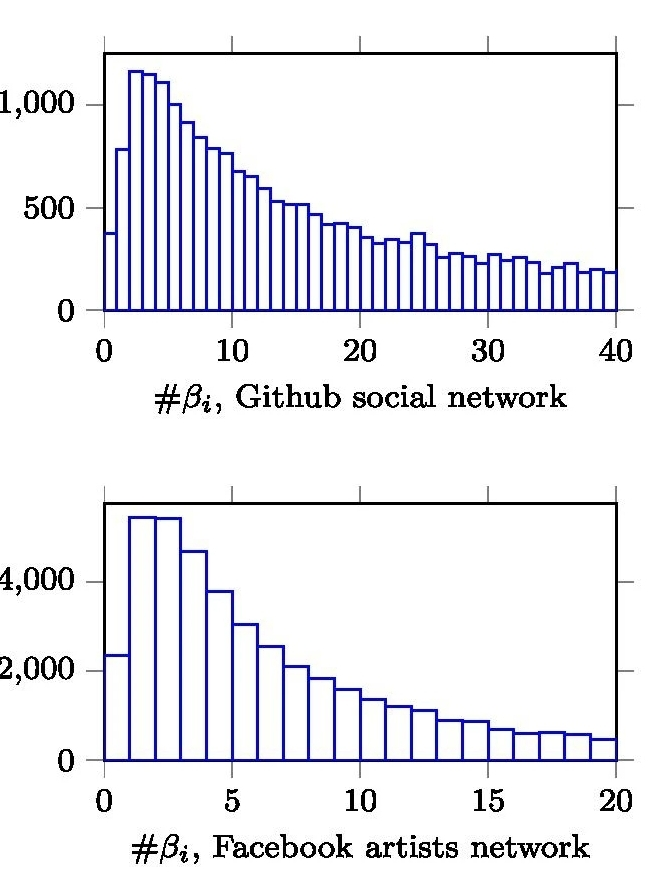
\includegraphics[scale=0.4]{examples1.jpg}
 \caption{Friendship index distributions in \\phone call network and Amazon delivery network}\label{fig:img3}
\end{figure}

\section{Implementation of the models}
In the course of the thesis, the following models were implemented: the standard Barabasi"--~Albert model, the Barabasi"--~Albert model with a Poisson distribution of initial degrees, and the triad closure model. All calculations were performed on a computer with an Intel core i5-8265U processor and 16 GB of RAM. The models were implemented in Python 3.9.1. The following libraries were used in the implementation: json, multiprocessing, random, and numpy. random.

All three implemented models are growing random graph models using the preferential attachment mechanism. In the implemented modifications, one vertex and a certain number $m$ of edges are added at each step. The $m$ parameter and the process of selecting neighbors of the new vertex depend on the model used. The triad closure model has an additional parameter $ p $. 

During the experiments we iterate over different models and different parameter values. In each experiment, a graph of 100,000 vertices is constructed. Since the resulting graphs are random, each graph is constructed ten times during the experiment, after which a histogram over the average ranges of values of the friendship index and the dynamics of the average friendship index of the graph are plotted.

In the implementation of models, the graph is represented by a pair of arrays \mintinline{py}{degrees} and \mintinline{py}{neibours}, which store the degree and the list of neighboring vertex numbers for each vertex of the graph, respectively. Each model is implemented in the form of function\\\mintinline{py}{model_name(n, args, funcs, dts)},\\where the parameter \mintinline{py}{n} sets the size of the final graph, the array \mintinline{py}{args} contains the model arguments, \mintinline{py}{funcs} is an array of metrics to be applied to the graph, and \mintinline{py}{dts} "--- frequency of applying metrics. 

Metrics are also represented by functions of the form\\\mintinline{py}{metric_name(degrees, neibours)},\\in which \mintinline{py}{degrees} is an array of degrees of graph vertices, and \mintinline{py}{neibours} is an array of arrays of neighboring vertices. In the course of our work, we used four metrics:
\begin{itemize}
\item \mintinline{py}{s(degrees, neibours)} "--- returns an array of sums of neighbor degrees for graph vertices.
\item \mintinline{py}{alfa(degrees, neibours)} "--- returns an array of average degrees of neighbors for graph vertices.
\item \mintinline{py}{beta(degrees, neibours)} "--- returns an array of friendship indices for graph vertices.
\item \mintinline{py}{mean_beta(degrees, neibours)} "--- returns the average friendship index of the entire graph
\end{itemize}
\subsection{Implementation of the standard Barabasi"--~Albert model}
The implementation of the standard Barabash model "--~ Albert is as follows. 

The model is implemented as a function\\
\mintinline{py}{my_bag(n, args, funcs, dts)},\\
as described above.

The null element of the \mintinline{py}{args} array is taken as the$ m $ parameter of the model. 

The implementation uses the array \mintinline{py}{ans}, which will store the values of the metrics of the constructed graph. Initially it is filled with empty arrays by the number of metrics: \linebreak\mintinline{py}{ans = [[] for _ in range(len(dts))]}.

A complete graph of $ m + 1$ vertices is created. To do this, the array \mintinline{py}{degrees} is filled with \mintinline{py}{m + 1} values \mintinline{py}{m} and the array \mintinline{py}{neibours} is formed from \mintinline{py}{m + 1} lists, each of which contains numbers of all currently existing vertices of the graph, except for the current one.
\begin{minted}{python}
		degrees = list(np.full(m + 1, m))
    neibours = [list(np.delete(np.arange(m + 1), i)) for i in np.arange(m + 1)]
\end{minted}
Next, two helper arrays are created: array \mintinline{py}{nodes} containing a list of the numbers of all vertices currently belonged to the graph, and \mintinline{py}{used} "--- an array that contains the vertices of the graph that are already attached to the new node. 
\begin{minted}{python}
		nodes = np.arange(m + 1)
    used = np.full(n, False)
\end{minted}

Then in a loop over $n - (m + 1)$ indexes new vertices are added to the graph. A list \mintinline{py}{conections} is formed to store the neighbors of the new node. The \mintinline{py}{random.choices} function selects $m$ unique vertices that are written to \mintinline{py}{conections}. The uniqueness of vertices is determined by the list \mintinline{py}{used}. The principle of preferential attachment is maintained by passing the degrees of vertices as an array of weights to \mintinline{py}{random. choices}.
\begin{minted}{python}
while j < m:
    choosen = random.choices(nodes, weights = degrees, k = 1)[0]
    if not used[choosen]:
        j += 1
        conections.append(choosen)
        used[choosen] = True
\end{minted}

In the next loop through the array elements \mintinline{py}{connections}  in the \mintinline{py}{used} array, all \mintinline{py}{True} are replaced with \mintinline{py}{False}. In addition, the values of the \mintinline{py}{neibours} list are supplemented with the links formed at this step, and the \mintinline{py}{degrees} array is changed accordingly. 
\begin{minted}{python}
for j in conections:
    used[j] = False
    neibours[i + 1].append(j)
    neibours[j].append(i)
    degrees[j] += 1
degrees.append(m)
\end{minted}

The last step in appending a new vertex in this algorithm is to collect graph metrics in the current state. For each function in the list \mintinline{py}{funcs}, the algorithm determines whether to measure this metric at the current step, based on the divisibility of \mintinline{py}{i} by the corresponding value \mintinline{py}{dts}. If the current metric is requested by the user at this step, the result of its calculation is added to the corresponding cell of the \mintinline{py}{ans} array. 
\begin{minted}{python}
for j in range(len(dts)):
    if i % dts[j] == 0:
        ans[j].append(funcs[j](degrees, neibours))
\end{minted}

The results of the entire \mintinline{py}{my_bag} function are placed in \mintinline{py}{ans}.

\subsection{Implementation of the Barabasi"--~Albert model with a random number of edges added at each iteration}
The implementation of the Barabasi"--~Albert model with a Poisson distribution of degrees of new vertices repeats the standard Barabasi"--~Albert model in many aspects. The first distinction lies in the contents of the parameter list \mintinline{py}{args}: instead of the $m$ parameter, this model accepts the $\lambda$ parameter for the Poisson distribution. This parameter is extracted to the variable \mintinline{py}{m} and used to generate the value \mintinline{py}{m0} "--- the number of vertices of the initial complete graph. 
\begin{minted}{python}
		m = args[0]
    ...
    m0 = np.random.poisson(m)
    degrees = list(np.full(m0 + 1, m0))
    neibours = [list(np.delete(np.arange(m0 + 1), i)) for i in np.arange(m0 + 1)]    
\end{minted}

The initial degrees of each new vertex are also determined according to the Poisson distribution. Since the degree of a new vertex can be neither greater than the number of nodes in the graph, nor less than one, then the number of neighbors of the new vertex must be subjected to appropriate restrictions.
\begin{minted}{python}
		mi = max(1, min(np.random.poisson(m), nodes.shape[0]))
\end{minted}
\subsection{Implementation of the triad closure model}
The triad closure model is also implemented as a modification of the standard Barabash model "--~Albert. Unlike other implemented models, the argument list contains two parameters: the fixed degree of new vertices $m$ and the probability of triad formation $p$. These parameters are extracted into variables with corresponding names.
\begin{minted}{python}
		m = args[0]
    p = args[1]
\end{minted}

Certain changes are also applied to the process of attaching new vertices: in this variation, there are two ways to select a candidate \mintinline{py}{choosen} for the role of a new neighbor of the current node. The choice based on the principle of preferential attachment is made either with probability $1-p$ from the set of all vertices of the graph, or from the number of neighbors of the vertex connected first. The first node is also attached according to the first option.
\begin{minted}{python}
if j == 0 or np.random.rand() > p:
    choosen = random.choices(nodes, weights = degrees, k = 1)[0]
else:
    choosen = random.choices(neibours[conections[0]], k = 1)[0]
\end{minted}
\subsection{Parallelized implementation of the Barabasi"--~Albert model}
To speed up the program, a multithreaded version of the algorithm was implemented using the multiprocessing and numpy libraries: the \mintinline{py}{run} function creates threads, distributes tasks and collects results, and the \linebreak \mintinline{py}{run_thread} function performs experiments in each thread separately and returns their results.

The function \mintinline{py}{run} takes seven arguments: the number of random graphs to construct, \mintinline{py}{N}; the number of threads \mintinline{python}{thread}, the algorithm for constructing a random graph \mintinline{python}{model}; the size of the graph \mintinline{python}{n}; array of model arguments \mintinline{python}{args}; list of metrics \mintinline{python}{funcs} and the frequency of their measurment \mintinline{python}{dts}. First, an object of the \mintinline{py}{multiprocessing.Manager} class is created, it will manage created threads. A reference to the dictionary with calculation results - \mintinline{py}{manager.dict()} is stored in the variable \mintinline{py}{res}. Then in a loop for each of \mintinline{py}{thread} cores \mintinline{py}{multiprocessing.Process} is created that will execute the corresponding thread. All processes are added to the list of running threads and started using the \mintinline{py}{p.start} method. Next, we wait for all threads to execute, collect all the results in the \mintinline{py}{ans} list, and return it as the result of the function.

At the first step in \mintinline{py}{run_thread} initializes an empty list \mintinline{py}{ans}. Then the specified number of random graphs is constructed, the specified metric is calculated for each of them, and the result is written to the \mintinline{py}{ans} list.
\begin{minted}{python}
def run_thread(N, i, res, model, n, args, funcs, dts):
    ans = []
    for j in range(N):
        ans.append(model(n, args, funcs, dts))
    res[i] = ans
def run(N, treads, model, n, args, funcs, dts):
    procs = []
    manager = multiprocessing.Manager()
    res = manager.dict()
    for i in range(treads):
        curn = min(N, math.ceil(N / (treads - i)))
        p = multiprocessing.Process(target=run_thread, args=(curn, i, res, model, n, args, funcs, dts))
        N -= curn
        procs.append(p)
        p.start()
    for proc in procs:
        proc.join()
    ans = []
    for i in res.values():
        ans += i
    return ans
\end{minted}
\subsection{Representation of the data for analysis}
This implementation contains a code snippet responsible for displaying data about the constructed graph for further analysis. The matplotlib, matplotlib.pyplot\cite{ptl} and numpy libraries are used for this purposes. 

During the experiments, the average friendship index of the graph vertices was measured for each model every 100 iterations, and after the graph was constructed, the friendship index for each vertex was calculated in order to display the distribution of its values. 

First, the data of the final friendship index is processed and presented as a three-dimensional array: for each constructed graph, for each measurment cycle, and for each vertex, there are values of the friendship index. Since data is sampled only once, the measurement axis can be removed, leaving only elements at null position. Then, a histogram is constructed for each graph, and the values of the histogram columns are averaged over the set of graphs. The average histogram is used to create a plot and the result is saved. 
\begin{minted}{python}
ans = run(10, 6, my_triad, n, [m, p], [beta, mean_beta], [n - 1, 100])
beta_data = np.array([i[0] for i in ans])
beta_data = [np.histogram(i[0], bins=100) for i in beta_data]
beta_data = [[i[0], np.delete(i[1], 100)] for i in beta_data]
beta_data = np.array(beta_data)
beta_data = beta_data.transpose((1, 2, 0))
beta_data = np.apply_along_axis(arr = beta_data, axis = 2, func1d = np.mean)
plt.bar(beta_data[1], beta_data[0])
plt.savefig('\\source\\repos\CSW\\diploma_results\\triad_beta_' + str(m) + '.jpg')
plt.clf()
\end{minted}

Similarly, information about the dynamics of the average friendship index is transformed. It is stored in the array \mintinline{py}{ans} under the index \mintinline{py}{1} and placed in the list \mintinline{python}{mean_beta_data}. Graph axis and tact axis are swaped. Then the data is averaged over the graphs, and a plot is constructed and saved from them.
\begin{minted}{python}
mean_beta_data = np.array([i[1] for i in ans])
mean_beta_data = np.apply_along_axis(arr=mean_beta_data, axis=2, func1d=lambda x: x[0])
mean_beta_data = mean_beta_data.transpose((1, 0))
mean_beta_data = np.apply_along_axis(arr=mean_beta_data, axis=1, func1d=mean)
plt.bar(mean_beta_data, np.arange(mean_beta_data.shape[0]))
plt.savefig('\\source\\repos\\CSW\\diploma_results\\triad_mean_beta_' + str(m) + '.jpg')
plt.clf()
\end{minted}

This sequence is repeated for each model of the graph, for each combination of parameters.
\begin{minted}{python}
for m in [3, 5]:
    for p in [0.25, 0.5, 0.75]:
  				ans = run(10, 6, my_triad, n, [m, p], [beta, mean_beta], [n - 1, 100])
      ...
      plt.clf()
for m in [3, 5]:
   		ans = run(10, 6, my_bag, n, [m, p], [beta, mean_beta], [n - 1, 100])
      ...
      plt.clf()
for m in [4, 5, 6]:
   		ans = run(10, 6, my_bag_poisson, n, [m, p], [beta, mean_beta], [n - 1, 100])
      ...
      plt.clf()
\end{minted}

In addition, you need to build and save one copy of each graph to a text document for further study. The json format was chosen as the text storage format for the graph, due to its structure, human readability, and ease of reading and writing. In the json file, the graph is represented as a list of dictionaries. Each element of the list represents a vertex of the graph. A vertex is represented by three dictionary entries: 
\begin{itemize}
\item \mintinline{js}{index} "--- index of a vertex in the graph,
\item \mintinline{js}{degree} "--- vertex degree, 
\item \mintinline{js}{neibours} "--- list of node neighbors. 
\end{itemize} 

Since graph construction algorithms do not return the entire graph, but only the values of the specified metrics, graph data must be extracted using the pseudometrics \mintinline{py}{d}, \mintinline{py}{neibours} and \mintinline{py}{index}. They return an array of degrees, a matrix of neighbors, and a list indexes of the graph, respectively. These values are saved to a file.
\begin{minted}{python}
def d (degrees, neibours):
    return degrees
def neibours (degrees, neibours):
    return neibours
def index (degrees, neibours):
    return np.arange(len(neibours))
...
						ans = run(1, 6, my_triad, n, [m, p], [index, d, neibours], [n - 1, n - 1, n - 1])
            ans = ans[0]
            ans = [i[0] for i in ans]
            prejson = [{'index':int(ans[0][i]), 'degree':int(ans[1][i]), 'neibours':[int(j) for j in ans[2][i]]} for i in range(len(ans[0]))]
            with open('\\source\\repos\\CSW\\diploma_results\\triad_graph_' + str(m) + '_' + str(p) + '.json', 'w') as f:
                json.dump(prejson, f)
                f.close()
    
\end{minted}

The result is a json file of the following format for each graph:
\begin{minted}{js}
[{"index": 0, "degree": 799, "neibours": [1, 2, ... , 99033]}, 
{"index": 1, "degree": 1032, "neibours": [0, 2, 3, ... , 99996]}, 
{"index": 2, "degree": 418, "neibours": [0, 1, 3, ... , 99864]}, 
{"index": 3, "degree": 624, "neibours": [0, 1, 2, ... , 99859]}, 
{"index": 4, "degree": 437, "neibours": [0, 1, 2, ... , 99922]}, 
{"index": 5, "degree": 174, "neibours": [4, 0, 1, 13, ... , 99982]},
...
{"index": 100000, "degree": 3, "neibours": [22224, 691, 5888]}]
\end{minted}
For the full program code, see\ref{app:program}.
\section{Graph analysis of real networks}
During the course of the thesis, several scripts were written for reading from a text file and analyzing graphs of real networks:
\begin{itemize}
\item script for efficiently reading large networks (up to several million vertices and tens of millions edges) and calculating the distribution of the friendship index in them.
\item program for reading graphs with information about the time when an edge appeared and tracking the dynamics of changes in the average friendship index.
\item script that reads two files: a file with edges and a file containing data about the time when a vertex was added, and also displays the dynamics of the average friendship index of the graph.
\end{itemize}
\subsection{Script for displaying the distribution of the friendship index}
Since the script for displaying the distribution of the friendship index must process large graphs with a limited amount of memory, it becomes impossible to save all the information about the graph. However, to calculate the friendship index, we need data about the neighbors of each vertex, because the graph is constantly changing during execution of the algorithm and it becomes impossible to calculate the friendship index when adding a vertex or updating it dynamically. This problem was solved by using two passes through the read file: one for counting the finite degrees of all vertices, and the second for transmitting this data to neighbors, since this algorithm does not imply storing data about the edges of the graph.

First, the script opens the necessary file for reading, creates a list for the values of the friendship index "--- \mintinline{py}{res} and a dictionary \mintinline{py}{degrees} for storing vertex degrees.
\begin{minted}{python}
file = open('\\source\\repos\\CSW\\real_graphs\\' + name + '.txt', 'r')
res = []
degrees = {}
\end{minted}
Then a read loop is started in which a line from the file is written to the variable \mintinline{py}{line}. If the line is equal to \mintinline{py}{null}, the loop is interrupted. Splitting the string \mintinline{py}{line} by a space character creates an edge \mintinline{py}{edge}. For each of the two ends of an edge, $1$ is added to the number of neighbors if there is no entry in \mintinline{py}{degrees}for the vertex yet then it is created and initialized $0$.
\begin{minted}{python}
while True:
    line = file.readline()
    if not line:
        break
    edge = [int(j) for j in line.split(" ")]
    if not edge[0] in degrees:
        degrees[edge[0]] = 0
    degrees[edge[0]] += 1
    if not edge[1] in degrees:
        degrees[edge[1]] = 0
    degrees[edge[1]] += 1
\end{minted}
The cursor is then moved to the beginning of the file. A dictionary \mintinline{py}{sum} is created for the sum of the neighbors of each vertex. And the second reading cycle starts, similar to the first one, with the only difference being that it counts the sums of neighbors, and not the degrees of vertices.
\begin{minted}{python}
file.seek(0)
sums = {}
while True:
    line = file.readline()
    if not line:
        break
    edge = [int(j) for j in line.split(" ")]
    if not edge[0] in sums:
        sums[edge[0]] = 0
    sums[edge[0]] += degrees[edge[1]]
    if not edge[1] in sums:
        sums[edge[1]] = 0
    sums[edge[1]] += degrees[edge[0]]
\end{minted}
At the end of the program, the friendship index is determined for each vertex, the file is closed, and then a histogram of the distribution of the friendship index in the specified graph is constructed and saved. 
\begin{minted}{python}
for i in degrees.keys():
        res.append(sums[i] / degrees[i] / degrees[i])
file.close()
bincnt = 100000
ans = np.histogram(res, bincnt)
x = ans[1]
y = ans[0]
x = np.resize(x, x.size - 1)
plt.bar(x[0:int(bincnt / 100 * 2)], y[0:int(bincnt / 100 * 2)])
plt.savefig("\\source\\repos\\CSW\\diploma_results\\" + name + "_static.jpg")
plt.clf()
\end{minted}
The full script code is provided in the Appendix~\ref{app:rgs}.
\subsection{Script for displaying the dynamics of the friendship index}
The script for displaying the dynamics of the friendship index must be able to repeatedly calculate the friendship index on the graph being read, so it saves not only lists of vertex neighbors, but also sums of neighbor degrees. 

The first steps are similar to the previous algorithm: the file is opened for reading and a reading cycle is started. However, data is written to the list \mintinline{py}{edge_list} almost without processing "--- the string is simply split by the character \mintinline{py}{\t}.
\begin{minted}{python}
file = open('\\source\\repos\\CSW\\real_graphs\\' + name, 'r')
    edge_list = []
    while True:
        line = file.readline()
        edge_list.append(line.split("\t"))
        if not line:
            break
    edge_list.pop()
\end{minted}
Then the elements \mintinline{py}{edge_list} are converted to triples of numbers containing the number of the first vertex of the edge, the number of the second vertex, and the unix time when the face was added. All data from the file is read and it closes.
\begin{minted}{python}
edge_list = [[i[0], 
              i[1], 
              datetime.datetime.strptime(i[3], '%Y-%m-%d %H:%M:%S').timestamp()] 
             for i in edge_list]
file.close()
\end{minted}
The resulting array is sorted using the \mintinline{py}{list.sort()} method in ascending timestamp order. The following variables are initialized:
\begin{itemize}
\item time measurement step \mintinline{py}{step}, 
\item time reference point \mintinline{py}{base}, 
\item list for storing results \mintinline{py}{res},
\item dictionaries that will contain the processed graph:
\subitem \mintinline{py}{degrees} "--- dictionary of graph degrees;
\subitem \mintinline{py}{neibours_degrees} "--- contains sums of degrees of neighbors.
\subitem \mintinline{py}{neibours} "--- sets of the vertex neighbors themselves.
\end{itemize}
\begin{minted}{py}
edge_list.sort(key = lambda i: i[2])
step = 1000
base = edge_list[0][2]
res = []
degrees = {}
neibours_degrees = {}
neibours = {}
\end{minted}
The next step in the loop through the sorted array is to check each vertex if it is present in the already described part of the graph. If there is no vertex yet, then entries in all three dictionaries are initialized for it.
\begin{minted}{python}
for i in edge_list:
    cnt += 1
    if not i[0] in degrees:
        degrees[i[0]] = 0
        neibours[i[0]] = set()
        neibours_degrees[i[0]] = 0
    if not i[1] in degrees:
        degrees[i[1]] = 0
        neibours[i[1]] = set()
        neibours_degrees[i[1]] = 0
\end{minted}
If the vertex is a loop, then the degree of one of the ends increases by $1$, the degree of the vertex itself is added to the sum of the degrees of the neighbors of this vertex, and the sum of the degrees of the neighbors of all adjacent vertices increases by $1$. Finally, an attempt is made to add a new vertex to the set of neighbors (obviously, the attempt will fail if the set already contains the node).
\begin{minted}{python}
if i[0] == i[1]:
    degrees[i[0]] += 1
    neibours_degrees[i[0]] += degrees[i[0]]
    for j in neibours[i[0]]:
        neibours_degrees[j] += 1
    neibours[i[0]].add(i[0])
\end{minted}
Othervise, the metioned steps are performed twice (for each end of the face).
\begin{minted}{python}
else:
  degrees[i[0]] += 1
  degrees[i[1]] += 1
  if not i[1] in neibours[i[0]] and not i[0] in neibours[i[1]]:
      neibours_degrees[i[0]] += degrees[i[1]]
      neibours_degrees[i[1]] += degrees[i[0]]
  for j in neibours[i[0]]:
      neibours_degrees[j] += 1
  for j in neibours[i[1]]:
      neibours_degrees[j] += 1
  neibours[i[0]].add(i[1])
  neibours[i[1]].add(i[0])
\end{minted}
When more than \mintinline{py}{step} seccond have passed since \mintinline{py}{base}, \mintinline{py}{base} is updated to the lowest value that exceeds the current time. The list \mintinline{py}{ans} records the index values of all graph vertices. These values are averaged using \mintinline{py}{numpy.mean()} and the average is added to \mintinline{py}{res}.
\begin{minted}{python}
if (i[2] - base) >= step:
    base = step * math.ceil(i[2] / step)
    ans = []
    for j in degrees.keys():
        ans.append(neibours_degrees[j] / degrees[j] / degrees[j])
    res.append(np.mean(ans))
\end{minted}
The \mintinline{py}{res} values are used to create and save a graph.
\begin{minted}{python}
plt.plot(res)
plt.savefig("\\source\\repos\\CSW\\diploma_results\\" + name + "_iterational_dynamics.jpg")
plt.clf()
\end{minted}
Since the script was not applied to very large graphs, there are still enough resources left during its execution to simultaneously process multiple networks in multithread mode.
\begin{minted}{python}
def run_thread(namegroup, i, res):
    ans = []
    for j in namegroup:
        ans.append(dynamics(j))
    res[i] = ans
def run(names):
    procs = []
    manager = multiprocessing.Manager()
    res = manager.dict()
    for (i, namegroup) in enumerate(names):
        p = multiprocessing.Process(target=run_thread, args=(namegroup, i, res))
        procs.append(p)
        p.start()
    for proc in procs:
        proc.join()
    ans = []
    for i in res.values():
        ans += i
    return ans
run([['askubuntu', 'askubuntu-a2q'], ['askubuntu-c2a', 'askubuntu-c2q'], ['mathoverflow', 'mathoverflow-a2q'], 
     ['mathoverflow-c2a', 'mathoverflow-c2q'], ['superuser', 'superuser-a2q'], ['superuser-c2a', 'superuser-c2q']])
\end{minted}
The full script code is provided in the Appendix~\ref{app:rg}.
\subsection{Script for displaying the dynamics of the friendship index in graphs presented in several files}
This program is a modification of the previous one. The main difference is that in this case, the time of adding vertices is read from a separate file in the dictionary \mintinline{py}{times}.
\begin{minted}{python}
time_file = open('\\source\\repos\\CSW\\real_graphs\\' + name + '-dates.txt', 'r')
times = {}
while True:
    line = time_file.readline()
    if not line:
        break
    line = line.split("\t")
    line = [int(line[0]), int(line[1].replace('-', ''))]
    times[line[0]] = line[1]
\end{minted}
In addition, the degree array \mintinline{py}{edge_list} is sorted using a lambda function that maps the vertex of the edge origin to the time it was added.
\begin{minted}{python}
edge_list.sort(key = lambda i: times[i[0]] if i[0] in times else 100000000)
\end{minted}
The full script code is provided in the Appendix~\ref{app:rgp}.
\section{Analysis}
In order to verify that the implemented models can act as models of social processes in the real world, it is necessary to show that the generated graphs have some properties of real networks. The friendship index was chosen as a characteristic for analysis
\[
\beta_i(t) = \dfrac{\alpha_i(t)}{deg_i(t)} = \dfrac{s_i(t)}{deg_i^2 (t)} = \dfrac{\sum_{j: (v_i, v_j ) \in E(t)} deg_j(t)}{deg_i^2 (t)}.
\]
The thesis considers the distribution of the friendship index and the dynamics of its average value.
\subsection{Analysis of the distribution and dynamics of the friendship index in the constructed graphs}
The graph shown in Fig.\,\ref{fig:bas3} shows the distribution of the friendship index in a graph constructed in accordance with standard Barabasi"---Albert model with the parameter $m = 3$. From this diagram, we can conclude that for the most vertices of the graph, the value of the friendship index is over 1. Therefore, the friendship paradox holds for this model. 
\begin{figure}[!ht]
\centering
\includegraphics[scale=0.7]{C:/Users/YURA/source/repos/CSW/diploma_results/static/ba_dist_beta_3.png}\\
\caption{Friendship index distribution in \\ standard Barabasi"---Albert model \\with $m=3$}\label{fig:bas3}
\end{figure}

Fig.\,\ref{fig:baps3} shows a graph of the distribution of the friendship index in a graph constructed using the modified Barabasi"---Albert model with the parameter $ m=4 $. Based on this graph, we can say that the friendship paradox is fulfilled in this model.
\begin{figure}[!ht]
\centering
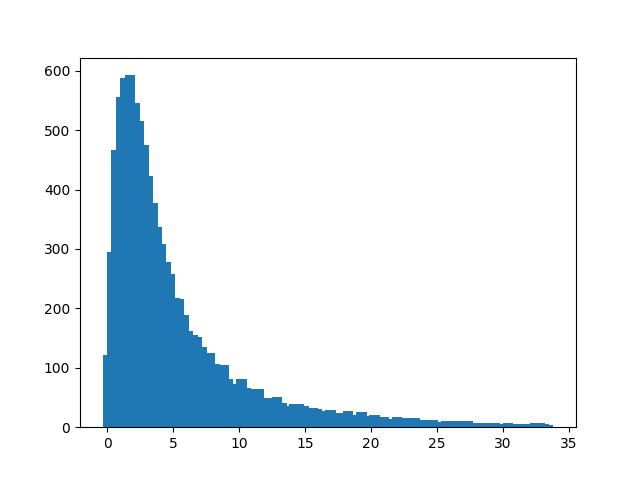
\includegraphics[scale=0.7]{C:/Users/YURA/source/repos/CSW/diploma_results/static/bap_dist_beta_3.png}\\
\caption{Distribution of the friendship index in \\modified Barabasi"---Albert model \\with $m=3$}\label{fig:baps3}
\end{figure}

The chart in Fig.\, \ref {fig:triads3} shows the distribution of the friendship index in the graph, which is based on the triad closure model. This graph also confirms the presence of the friendship paradox in the model under consideration.
\begin{figure}[!ht]
\centering
\includegraphics[scale=0.7]{C:/Users/YURA/source/repos/CSW/diploma_results/static/triad_dist_beta_3_0.25.png}\\
\caption{Friendship index distribution in\\triad closure model\\with $m=3$ and $ p=0.25 $}\label{fig:triads3}
\end{figure}

In Fig.\,\ref{fig:basl3}, \ref{fig:bapsl3}, \ref{fig:triadsl3} output the same values, but on the logarithmic scale. In accordance with the graph, we can hypothesize that the distribution of the values of the friendship index occurs in accordance with a power function
\[
y = (\alpha \cdot x)^\gamma.
\]
\begin{figure}[!ht]
\centering
\includegraphics[scale=0.7]{C:/Users/YURA/source/repos/CSW/diploma_results/static_log/ba_dist_beta_3.png}\\
\caption{Distribution of the friendship index in the \\standard Barabasi"---Albert model \\with $m=3$, on the logarithmic scale}\label{fig:basl3}
\end{figure}
\begin{figure}[!ht]
\centering
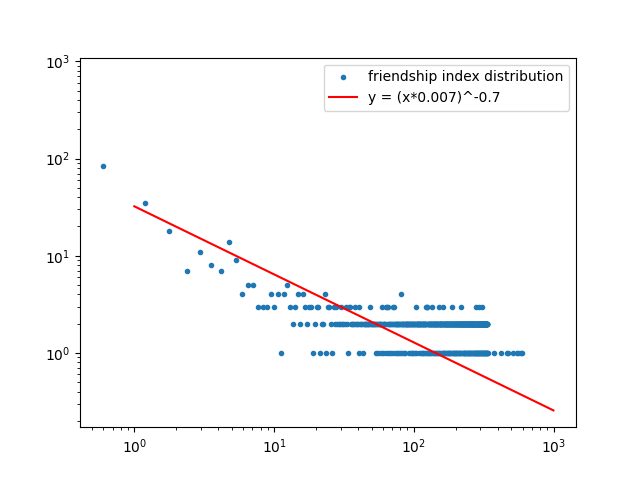
\includegraphics[scale=0.7]{C:/Users/YURA/source/repos/CSW/diploma_results/static_log/bap_dist_beta_4.png}\\
\caption{Distribution of the friendship index in \\modified Barabasi"---Albert model \\with $m=4$, on the logarithmic scale}\label{fig: bapsl3}
\end{figure}
\begin{figure}[!ht]
\centering
\includegraphics[scale=0.7]{C:/Users/YURA/source/repos/CSW/diploma_results/static_log/triad_dist_beta_3_0.25.png}\\
\caption{Friendship index distribution in \\triad closure model\\with $m=3$ and $ p=0.25 $, on the logarithmic scale}\label{fig:triadsl3}
\end{figure}

Graphs of the friendship index distribution in these models with other parameters $ m $ and $ p $ are presented in Appendix~\ref{app:dist}.

Figure\,\ref{fig:badl3} contains a diagragram in logarithmic scale of the dynamics of the average friendship index in the Barabasi"---Albert model at $m=3$ in comparison with the plot of a power function
\[
y=(10000 \cdot x)^{0.12}.
\]
Based on this graph, we can assume that the average value of the friendship index in the models under consideration grows in accordance with the power function. 
\begin{figure}[!ht]
\centering
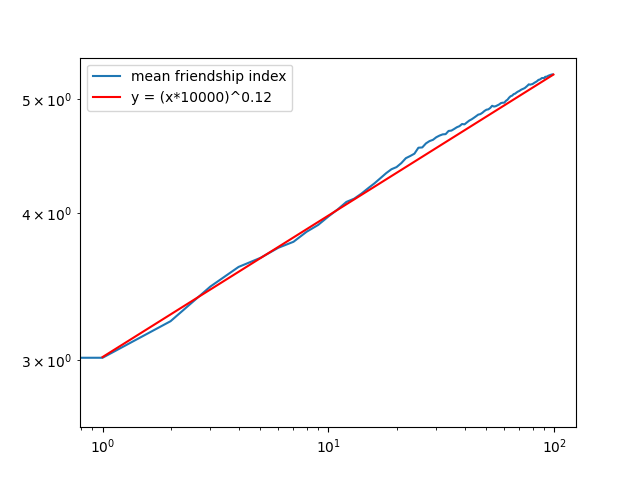
\includegraphics[scale=0.7]{C:/Users/YURA/source/repos/CSW/diploma_results/dynamic_log/ba_mean_beta_3.png}\\
\caption{Dynamics of the average value of the friendship index in the \\standard Barabasi"---Albert model \\with $m=3$, on the logarithmic scale}\label{fig:badl3}
\end{figure}

The chart of the dynamics of the average friendship index in the Barabasi"---Albert model with the Poisson distribution of the initial degrees of vertices with $m=4$ on the logarithmic scale, is shown in Fig.\, \ref{fig:bapdl3}, coincides with the plot of the power function
\[
y=(80000 \cdot x)^{0.13}.
\]
\begin{figure}[!ht]
\centering
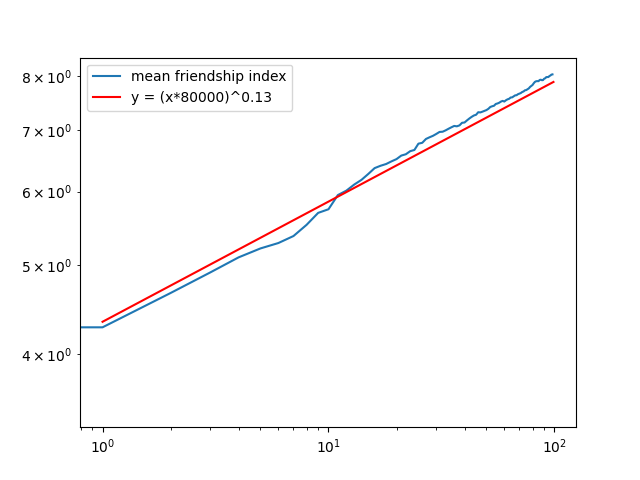
\includegraphics[scale=0.7]{C:/Users/YURA/source/repos/CSW/diploma_results/dynamic_log/bap_mean_beta_4.png}\\
\caption{Dynamics of the average value of the friendship index in \\modified Barabasi"---Albert model \\with $m=4$, on the logarithmic scale}\label{fig: bapdl3}
\end{figure}

Figure\, \ref{fig:triaddl3} shows a plot of the dynamics of the average friendship index in the triad closure model at $m=3$ and $ p=0.25 $ on the logarithmic scale, which is identical to the power function:
\[
y=(40000 \cdot x)^{0.11}.
\]
\begin{figure}[!ht]
\centering
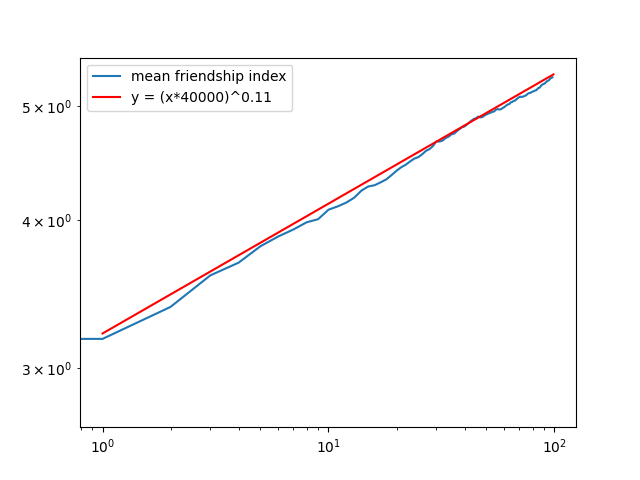
\includegraphics[scale=0.7]{C:/Users/YURA/source/repos/CSW/diploma_results/dynamic_log/triad_mean_beta_3_0.25.png}\\
\caption{Dynamics of the average value of the friendship index in the \\triad closure model\\with $m=3$, on the logarithmic scale}\label{fig:triaddl3}
\end{figure}

Diagrams of the friendship index dynamics in other models are presented in the appendix~\ref{app:dyn}.
\subsection{Analysis of the distribution and dynamics of the friendship index in real networks}	
In the course of the tesis, graphs of the following networks from the real world were considered:
\begin{itemize}
\item LiveJournal
\item Twitter
\item Reddit
\item Google+
\item askubuntu
\item mathoverflow
\item superuser
\item citation network for articles in the field of high energy physics phenomenology
\item internal social network of the University of California, Irvine
\end{itemize}
\subsubsection{Analysis of the distribution of the friendship index in the LiveJournal social network}
LiveJournal (LJ) is a blog platform for keeping online diaries (blogs), as well as a separate personal blog hosted on this platform. Provides an opportunity to publish your own and comment on other people's posts, run collective blogs ("communities"), add other users to friends ("friend") and follow their posts in the "friends feed" ("friendlent").

The thesis contemplates a dataset based on the state of the LiveJournal platform in 2009 and presented in \cite{lj}. In the graph, users act as vertices, and the presence of an edge between the vertices indicates a friendship relationship between the corresponding users. The graph contains $4\, 847\, 571 $ nodes and $68\, 993\, 773$ edges, which makes it too large to consider the growth dynamics of the average friendship index, but on the other hand, it allows us to study the distribution of the friendship index in a large graph. 

Fig. \ref{fig:lj} shows a diagram of the distribution of the friendship index in the described graph. We can assume that the friendship index is distributed according to the power law
\[
y = (0.000002 \cdot x)^{-2}.
\]
Note that the similarity with the power law of distribution of values is also observed in graphs constructed in accordance with the models of random graphs considered earlier in this paper.

\begin{figure}[!ht]
\centering
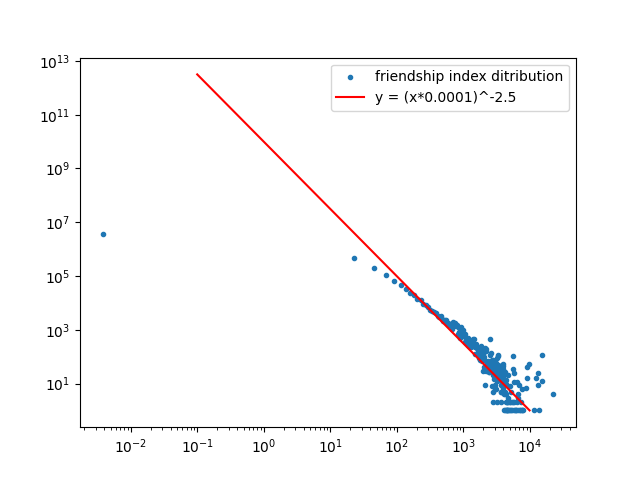
\includegraphics[scale=0.7]{C:/Users/YURA/source/repos/CSW/diploma_results/static_real_log/soc-LiveJournal1.png}\\
\caption{Distribution of the friendship index in\\social network <<LiveJournal>>\\on the logarithmic scale}\label{fig:lj}
\end{figure}

\subsubsection{Analysis of the distribution of the friendship index in the Twitter social network}
Twitter is an American microblogging service and social network where users post messages known as "tweets" and interact with them. Users interact with Twitter through a browser, mobile app, or API. Until April 2020, the services were available via SMS. The service is provided by Twitter, Inc., which is based in San Francisco, California, and has more than 26 offices worldwide.  In 2013, it entered the top ten most visited sites and was named "SMS of the Internet". By the beginning of 2019, Twitter had more than 330 million monthly active users. In practice, the vast majority of tweets are written by a minority of users. 

Data about this network is taken from \cite{twit}. The graph describes the relationship of friendship between confirmed users belonging to certain circles such as: <<artists>>, <<politicians>>, etc. It contains $81\,306$ vertices connected by $1\,768\,149$ edges. On the graph shown in Fig.\,\ref{fig:twit}, it can be found that the distribution of the friendship index in this network does not correspond well to the power function.

\begin{figure}[!ht]
\centering
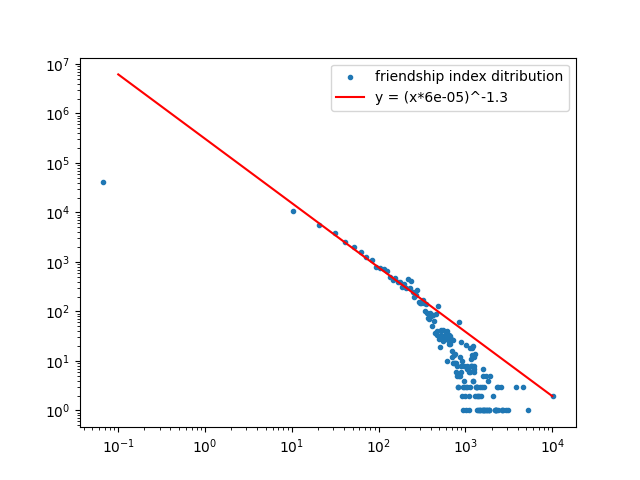
\includegraphics[scale=0.7]{C:/Users/YURA/source/repos/CSW/diploma_results/static_real_log/twitter_combined.png}\\
\caption{Distribution of the friendship index in\\social network <<Twitter>>\\on the logarithmic scale}\label{fig:twit}
\end{figure}

In this case dynamics of the friendship index also was not possible to be calculated.

\subsubsection{Analysis of the distribution and dynamics of the friendship index in the citation network of articles in the field of high energy physics phenomenology}
The data set contains information on $34\,546$ high-energy physics articles published from January 1993 to April 2003 on arXiv.org "--- electronic archive with open access for scientific articles and preprints in physics, mathematics, astronomy, computer science, biology, electrical engineering, statistics, financial mathematics and economics. The graph contains $421\,578$ edges. The dataset was introduced in \cite{cit}.

Figure\,\ref{fig:cits} shows the distribution of the friendship index in this network. From this plot, we can assume that the friendship index in the citation network, like the friendship index in the reviewed random graphs, is distributed according to the power law
\[
y = (0.0055 \cdot x)^{-2}
\].
\begin{figure}[!ht]
\centering
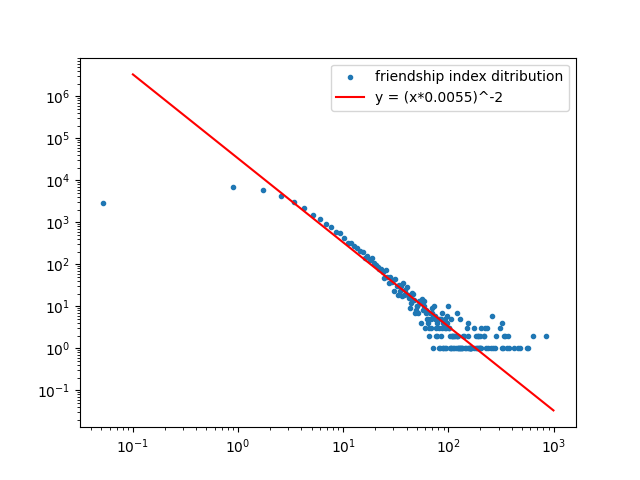
\includegraphics[scale=0.7]{C:/Users/YURA/source/repos/CSW/diploma_results/static_real_log/Cit-HepPh.png}\\
\caption{Distribution of the friendship index in the \\citation network\\on the logarithmic scale}\label{fig:cits}
\end{figure}

A diagram of the dynamics of the friendship index in this network is shown in Fig.\,\ref{fig: citd}. We can hypothesize that the average value of the friendship index in the graph grows in accordance with the power function
\[
y = (11000 \cdot x)^{0.12}.
\]
This, in terms of this assumption, corresponds to the rate of growth of the friendship index in the networks of the Barabasi"---Albert and triad closure models.
\begin{figure}[!ht]
\centering
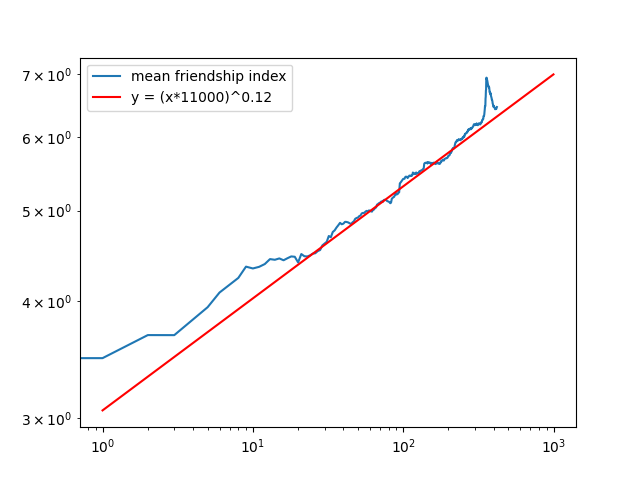
\includegraphics[scale=0.7]{C:/Users/YURA/source/repos/CSW/diploma_results/dynamic_real_log/cit-HepPh_mean.png}\\
\caption{Dynamics of the friendship index in the \\citation network\\on the logarithmic scale}\label{fig: citd}
\end{figure}

\subsubsection{Analysis of the distribution and dynamics of the friendship index in the Reddit forum network}
Reddit is a site that combines the features of a social network and a forum, where registered users can post links to any information they like on the Internet and discuss it. Like many other similar sites, Reddit supports a voting system for liked posts � the most popular ones appear on the main page of the site. One of the most popular sites in the world � 20th place in terms of traffic according to SimilarWeb. 

In this case, we consider a network of hyperlinks between subreddits (communities on <<Reddit>>) data was collected over two and a half years: from January 2014 to April 2017. The graph consists of $55\,863$ nodes connected by$ 858\,490$ edges. The data was submitted in \cite{reddit}.

Figure\, \ref{fig:reds} shows a chart of distribution of the friendship index in the hyperlink graph between subreddits. From the graph, we can assume that the distribution of the friendship index in this network also corresponds to a power function, which in this case looks like this:
\[
y = (2e^{-6} \cdot x)^{-1}.
\]
\begin{figure}[!ht]
\centering
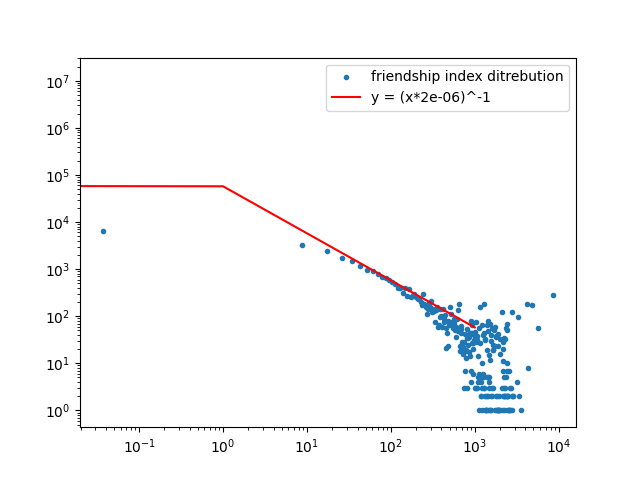
\includegraphics[scale=0.7]{C:/Users/YURA/source/repos/CSW/diploma_results/static_real_log/soc-redditHyperlinks-body.png}\\
\caption{Distribution of the friendship index in \\Reddit forum network\\on the logarithmic scale}\label{fig:reds}
\end{figure}

Figure\, \ref{fig:redd} indicates that the diagram of the friendship index dynamics on the Reddit forum is similar to the graph of the power function
\[
y = (0.03 \cdot x)^{0.8}.
\]
\begin{figure}[!ht]
\centering
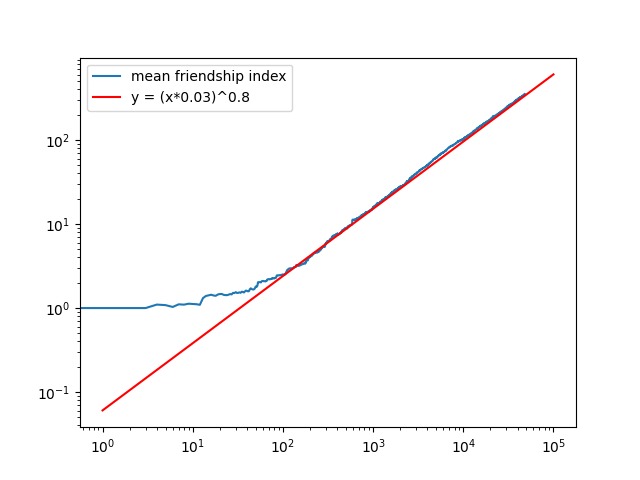
\includegraphics[scale=0.7]{C:/Users/YURA/source/repos/CSW/diploma_results/dynamic_real_log/soc-redditHyperlinks-body_mean.png}\\
\caption{Dynamics of the friendship index in the \\Reddit forum network\\on the logarithmic scale}\label{fig:redd}
\end{figure}

\subsubsection{Analysis of the distribution and dynamics of the friendship index in the AskUbuntu Q\&A system}
AskUbuntu "--- a website for working with questions and answers that arise when using the Ubuntu Linux distribution. Sites allow users to ask and answer questions. By taking into account activities, voting takes place for questions and answers, positive and negative. You can edit questions and answers in wiki mode. All materials published online are available under the free CC BY-SA license. 

4 datasets were reviewed: 
\begin{itemize}
\item graph of answers to the questions, which consists of$ 137\,517 $ vertices representing users, and $280\,102$ connections between them. the connection between users $A$ and $B$ is that user $A$ answered the user's question $B$;
\item a question citation graph containing $79\,155$ nodes and $327\,513$ edges, where a directed edge is drawn between the user and the author of the question that they cited.
\item response citation graph consisting of $75\,555$ and $356\,822$ vertices and edges, respectively, an edge is drawn from the user who referred to the answer to the user who wrote it.
\item and a general graph containing all users and all edges of all previous graphs, with $159\,316$ nodes and $964\,437$ connections.
\end{itemize}
Data for these graphs have been collected for more than seven years, and they were presented in the article \cite{au}.

The properties of this network do not fully correspond to the behavior of the models studied in the thesis: in Fig.\,\ref{fig:aus}, you can see that the distribution of the friendship index does not correspond well to the power function and, therefore, does not correspond to the constructed models.

\begin{figure}[!ht]
\centering
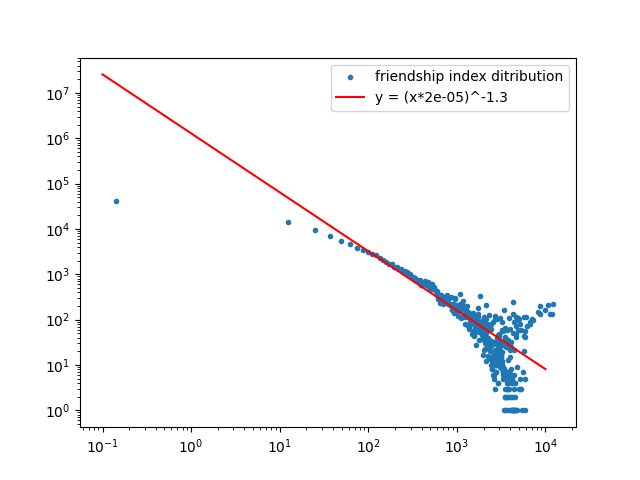
\includegraphics[scale=0.7]{C:/Users/YURA/source/repos/CSW/diploma_results/static_real_log/sx-askubuntu.png}\\
\caption{Distribution of the friendship index in the \\AskUbuntu network\\on the logarithmic scale}\label{fig:aus}
\end{figure}

However, the average value of the friendship index, as in models of random graphs, grows rather accordingly to the power law
\[
y = (0.8 \cdot x)^{0.5},
\]
as shown in the chart \ref{fig:aud}.
\begin{figure}[!ht]
\centering
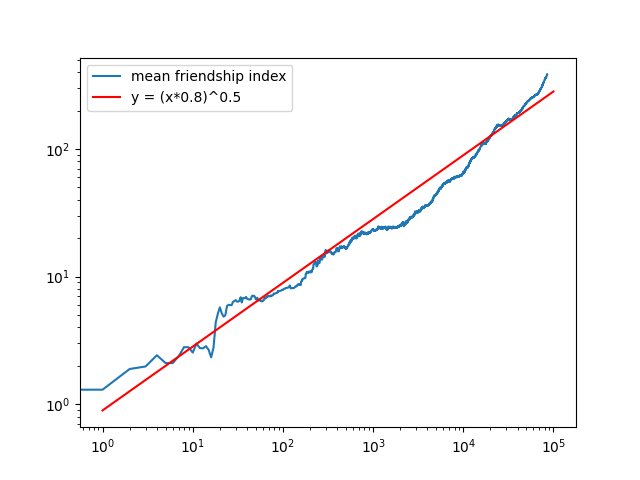
\includegraphics[scale=0.7]{C:/Users/YURA/source/repos/CSW/diploma_results/dynamic_real_log/sx-askubuntu_mean.png}\\
\caption{Dynamics of the friendship index in the \\AskUbuntu network\\on the logarithmic scale}\label{fig:aud}
\end{figure}

These patterns are most clearly shown in the graph of the network of answers to questions. Plots of the distribution and dynamics of the index for this network are shown in Fig.\,\ref{fig:auaqs} and \ref{fig:auaqd}, respectively.

\begin{figure}[!ht]
\centering
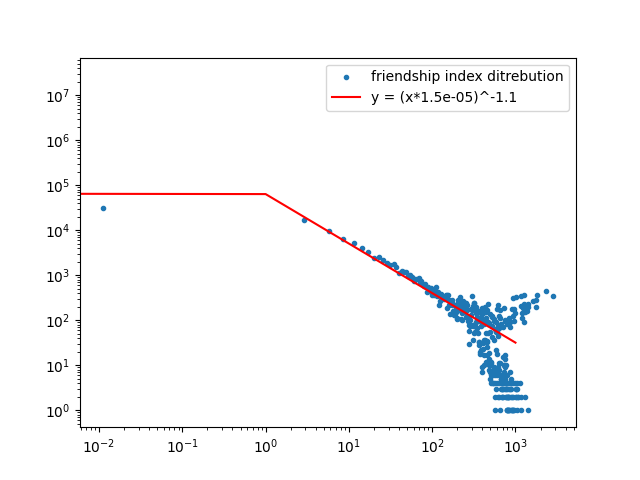
\includegraphics[scale=0.7]{C:/Users/YURA/source/repos/CSW/diploma_results/static_real_log/sx-askubuntu-a2q.png}\\
\caption{Distribution of the friendship index in \\The AskUbuntu question answer network\\on the logarithmic scale}\label{fig:auaqs}
\end{figure}

\begin{figure}[!ht]
\centering
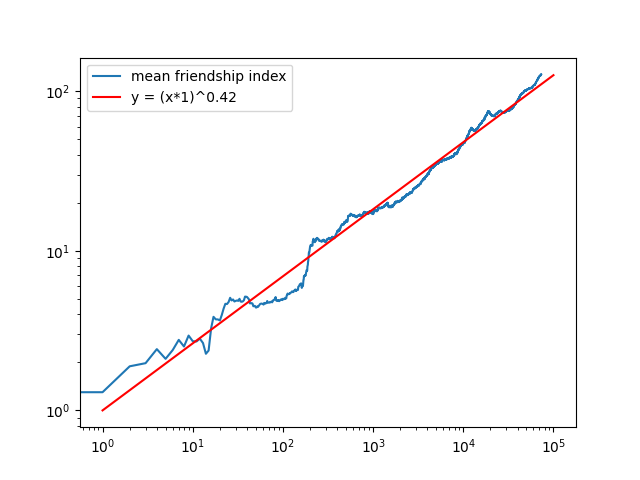
\includegraphics[scale=0.7]{C:/Users/YURA/source/repos/CSW/diploma_results/dynamic_real_log/sx-askubuntu-a2q_mean.png}\\
\caption{Dynamics of the friendship index in the \\network of answers to questions on AskUbuntu\\on the logarithmic scale}\label{fig:auaqd}
\end{figure}

Graphs of other subnets are shown in the Appendix~\ref{app:real}

\subsubsection{Analysis of the distribution and dynamics of the friendship index in the SuperUser Q\&A system}
SuperUser, like AskUbuntu, is a Q\&A platform, and unlike the previous network, it is dedicated to computer enthusiasts. Like AskUbuntu, it acts as one of the sections of StackExchange and it follows the same basic network rules: anyone can ask a question, anyone can answer it, and anyone can vote for the answer or question.

Three subnets were also allocated for this network:
\begin{itemize}
\item question answers network
\item question citation network
\item response citation network
\end{itemize}
The data were also presented in \cite{au}.

The network of the SuperUser platform does not follow the patterns identified in random graphs in the course of this work. In Fig.\,\ref{fig:sus}, it can be seen that the plot of the distribution of the friendship index rather poorly coincides with the power function, as well as the diagram of the dynamics of the friendship index presented in Fig.\,\ref{fig:sud}.
\begin{figure}[!ht]
\centering
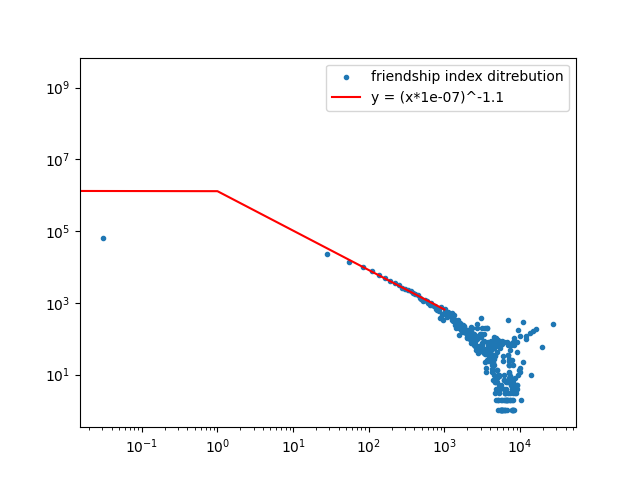
\includegraphics[scale=0.7]{C:/Users/YURA/source/repos/CSW/diploma_results/static_real_log/sx-superuser.png}\\
\caption{Distribution of the friendship index in \\SuperUser network\\on the logarithmic scale}\label{fig:sus}
\end{figure}
\begin{figure}[!ht]
\centering
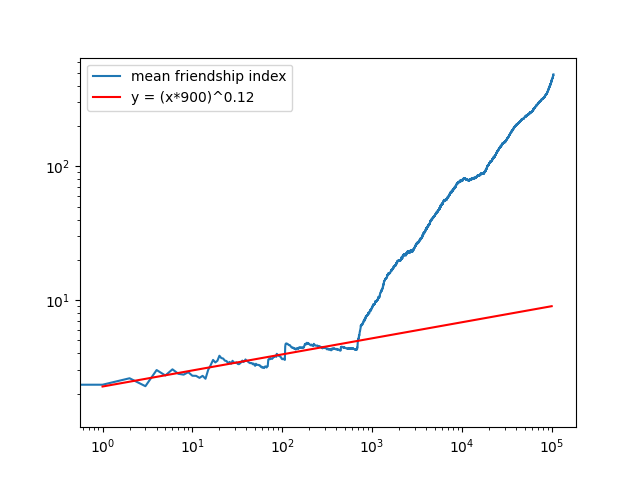
\includegraphics[scale=0.7]{C:/Users/YURA/source/repos/CSW/diploma_results/dynamic_real_log/sx-superuser_mean.png}\\
\caption{Dynamics of the friendship index in \\SuperUser network\\on the logarithmic scale}\label{fig:sud}
\end{figure}

In the question citation network, this deviation only increases, as can be seen in the graphs \ref{fig:sucqs} and \ref{fig:sucqd}.
\begin{figure}[!ht]
\centering
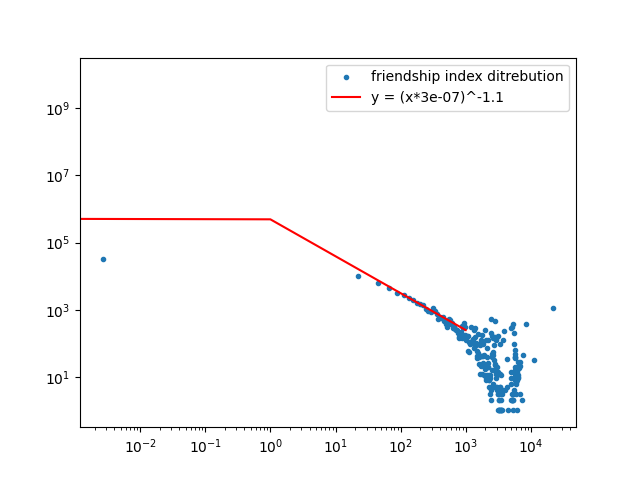
\includegraphics[scale=0.7]{C:/Users/YURA/source/repos/CSW/diploma_results/static_real_log/sx-superuser-c2q.png}\\
\caption{Distribution of the friendship index in \\The SuperUser question citation network\\on the logarithmic scale}\label{fig:sucqs}
\end{figure}
\begin{figure}[!ht]
\centering
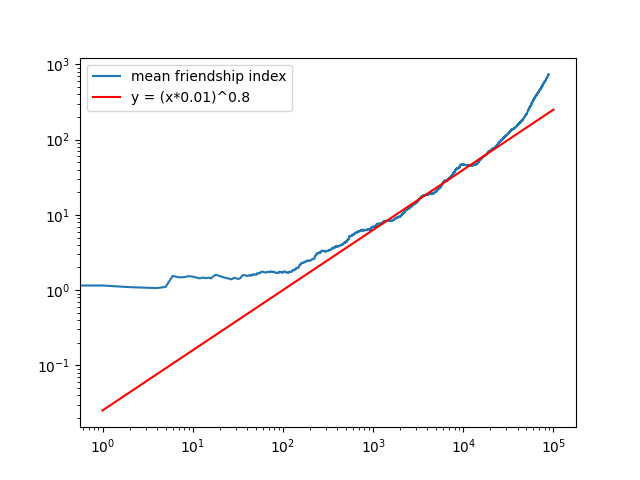
\includegraphics[scale=0.7]{C:/Users/YURA/source/repos/CSW/diploma_results/dynamic_real_log/sx-superuser-c2q_mean.png}\\
\caption{Dynamics of the friendship index in \\The SuperUser question citation network\\on the logarithmic scale}\label{fig:sucqd}
\end{figure}

At the same time, in the sub-network of answers to questions, the dynamics of the friendship index still probably obeys the power law, which can be observed in Fig.\,\ref{fig:suaqd}.
\begin{figure}[!ht]
\centering
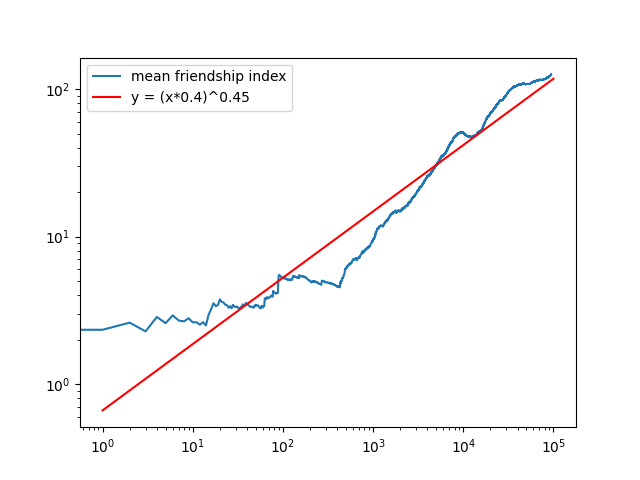
\includegraphics[scale=0.7]{C:/Users/YURA/source/repos/CSW/diploma_results/dynamic_real_log/sx-superuser-a2q_mean.png}\\
\caption{Dynamics of the friendship index in \\The SuperUser question answer network\\on the logarithmic scale}\label{fig:suaqd}
\end{figure}

Graphs for the remaining subnets are presented in the \ref{app:real} app. There are also graphs of the distribution and dynamics of the friendship index in Google+, MathOverflow, and student messages network of the University of California in Irvine, data for which were taken from the works \cite{twit}, \cite{au}, and \cite{stdmsg}. In the\ref{tab table:general} a comparative analysis of all the considered networks is presented.
\begin{table}[!ht]
\small
\caption{Summary table of experimental results}\label{tab:general}
\begin{tabular}{>{\raggedright}p{7cm}@{\ }>{\centering}p{3cm}@{\ }>{\centering}p{1.1cm}@{\ }>{\centering}p{3cm}@{\ }>{\centering}p{1cm}}
\hline\noalign{\smallskip}
\centering Network&Friendship Index Distribution Function&$\gamma_{ dist }$&Friendship Index Dynamics Function&$\gamma_{ dyn }$\cr
\noalign{\smallskip}\hline\noalign{\smallskip}
Barabasi"---Albert model at $m=3$&power-law&-0.7&power-law&0.15\cr
Barabasi"---Albert model at $m=3$&power-law&-0.7&power-law&0.15\cr
Barabasi"---Albert model with Poisson distribution of initial degrees at $m=4$&power&-0.5&power&0.15\cr
Barabasi"---Albert model with Poisson distribution of initial degrees at $m=5$&power&-0.5&power&0.15\cr
Barabasi"---Albert model with Poisson distribution of initial degrees at $m=6$&power&-0.45&power&0.15\cr
Triad closure model for $m=3$ and $p=0.25$&power&-0.7&power&0.15\cr
Triad closure model for $m=3$ and $p=0.5$&power-law&-0.7&power-law&0.15\cr
Triad closure model for $m=3$ and $p=0.75$&power&-0.4&power&0.12\cr
Triad closure model for $m=5$ and $p=0.25$&power-law&-0.6&power-law&0.13\cr
Triad closure model for $m=5$ and $p=0.5$&power-law&-0.6&power-law&0.13\cr
Triad closure model for $m=5$ and $p=0.75$&power&-0.55&power&0.12\cr \cr
Twitter&unknown function&N/A&N/A&N/A\cr
Google+&power-law&-1.7&N/A&N/A\cr
Reddit&power&-1.2&power&0.8\cr
AskUbuntu&unknown function&N/A&power function&0.5\cr
MathOverflow&power-law&-1.2&power-law&0.45\cr
SuperUser&unknown function&N/A&exponential&N/A\cr
Citation Network&power&-2&power&0.12\cr
LiveJournal&Power&-2.5&N/A&N/A\cr
Student Message Network&Power&-0.9&Power&0.5\cr
\noalign{\smallskip}\hline
\end{tabular}
\end{table}

% Conclusion section
\conclusion
During the course of the thesis, various models of generating growing networks were studied. And the following random graph generation models were implemented:
\begin{itemize}
\item standard Barabasi"--~Albert model; 
\item Barabasi"--~Albert model with Poisson distribution of initial degrees of nodes; 
\item the triad closure model.
\end{itemize} 

A series of experiments was conducted in which random graphs were constructed according to the implemented models,  and the dynamics of the average value of the friendship index in the network and the distribution of the values of the friendship index in the final graph were studied. In accordance with the results obtained, it is hypothesized that the distribution of the friendship index of the vertices of the final graph and the growth of the average value of the friendship index during the formation of the network occurs according to the power law.  

The values of the distribution of the friendship index and the growth dynamics of the average value of the friendship index in a number of real networks were studied. It is concluded that for most networks, the behavior of the friendship index is similar to its behavior in networks growing according to the studied models.

The models were implemented and experiments were performed using Python with the json, multiprocessing, pyplot, numpy, and random libraries.


% List of references
\bibliographystyle{gost780uv}
\bibliography{thesis}

% End of main document and start of appendices
% Each subsequent section of the document will be an attachment

\appendix
\section{Text of the program}\label{app:program}
This appendix contains the full text of the implementation of the Barabasi"--~Albert model.
\begin{minted}{python}
from multiprocessing.dummy import current_process
from statistics import mean

import matplotlib as mpl
import matplotlib.pyplot as plt
import math
import random
import pylab
import multiprocessing
import datetime
import numpy as np
import json

def my_bag_poisson(n, args, funcs, dts):
    m = args[0]
    ans = [[] for _ in range(len(dts))]
    m0 = np.random.poisson(m)
    degrees = list(np.full(m0 + 1, m0))
    neibours = [list(np.delete(np.arange(m0 + 1), i)) for i in np.arange(m0 + 1)]
    nodes = np.arange(m0 + 1)
    used = np.full(n, False)
    for i in range(m0, n):
        mi = max(1, min(np.random.poisson(m), nodes.shape[0]))
        conections = []
        j = 0
        while j < mi:
            choosen = random.choices(nodes, weights = degrees, k = 1)[0]
            if not used[choosen]:
                j += 1
                conections.append(choosen)
                used[choosen] = True
        neibours.append([])
        for j in conections:
            used[j] = False
            neibours[i + 1].append(j)
            neibours[j].append(i)
            degrees[j] += 1
        degrees.append(mi)
        nodes = np.append(nodes, nodes.shape[0])
        for j in range(len(dts)):
            if i % dts[j] == 0:
                ans[j].append(funcs[j](degrees, neibours))
    return ans

def my_triad(n, args, funcs, dts):
    m = args[0]
    p = args[1]
    ans = [[] for _ in range(len(dts))]
    degrees = list(np.full(m + 1, m))
    neibours = [list(np.delete(np.arange(m + 1), i)) for i in np.arange(m + 1)]
    nodes = np.arange(m + 1)
    used = np.full(n, False)
    for i in range(m, n):
        conections = []
        j = 0
        while j < m:
            if j == 0 or np.random.rand() > p:
                choosen = random.choices(nodes, weights = degrees, k = 1)[0]
            else:
                choosen = random.choices(neibours[conections[0]], k = 1)[0]
            if not used[choosen]:
                j += 1
                conections.append(choosen)
                used[choosen] = True
        neibours.append([])
        for j in conections:
            used[j] = False
            neibours[i + 1].append(j)
            neibours[j].append(i)
            degrees[j] += 1
        degrees.append(m)
        nodes = np.append(nodes, nodes.shape[0])
        for j in range(len(dts)):
            if i % dts[j] == 0:
                ans[j].append(funcs[j](degrees, neibours))
    return ans


def my_bag(n, args, funcs, dts):
    m = args[0]
    ans = [[] for _ in range(len(dts))]
    degrees = list(np.full(m + 1, m))
    neibours = [list(np.delete(np.arange(m + 1), i)) for i in np.arange(m + 1)]
    nodes = np.arange(m + 1)
    used = np.full(n, False)
    for i in range(m, n):
        conections = []
        j = 0
        while j < m:
            choosen = random.choices(nodes, weights = degrees, k = 1)[0]
            if not used[choosen]:
                j += 1
                conections.append(choosen)
                used[choosen] = True
        neibours.append([])
        for j in conections:
            used[j] = False
            neibours[i + 1].append(j)
            neibours[j].append(i)
            degrees[j] += 1
        degrees.append(m)
        nodes = np.append(nodes, nodes.shape[0])
        for j in range(len(dts)):
            if i % dts[j] == 0:
                ans[j].append(funcs[j](degrees, neibours))
    return ans

def run_thread(N, i, res, model, n, args, funcs, dts):
    ans = []
    for j in range(N):
        ans.append(model(n, args, funcs, dts))
    res[i] = ans
def run(N, treads, model, n, args, funcs, dts):
    procs = []
    manager = multiprocessing.Manager()
    res = manager.dict()
    for i in range(treads):
        curn = min(N, math.ceil(N / (treads - i)))
        p = multiprocessing.Process(target=run_thread, args=(curn, i, res, model, n, args, funcs, dts))
        N -= curn
        procs.append(p)
        p.start()
    for proc in procs:
        proc.join()
    ans = []
    for i in res.values():
        ans += i
    return ans
def d (degrees, neibours):
    return degrees
def neibours (degrees, neibours):
    return neibours
def index (degrees, neibours):
    return np.arange(len(neibours))
def s (degrees, neibours):
    return [sum([degrees[i] for i in j]) for j in neibours]
def alfa (degrees, neibours):
    return [si / di for (si, di) in zip(s(degrees, neibours), d(degrees, neibours))]
def beta (degrees, neibours):
    return [ai / di for (ai, di) in zip(alfa(degrees, neibours), d(degrees, neibours))]
def mean_beta (degrees, neibours):
    return [mean(beta(degrees, neibours))]

if __name__ == "__main__":
    n = 100000
    m = 5
    p = 0.25
    
    for m in [3, 5]:
        for p in [0.25, 0.5, 0.75]:
            ans = run(1, 6, my_triad, n, [m, p], [index, d, neibours], [n - 1, n - 1, n - 1])
            ans = ans[0]
            ans = [i[0] for i in ans]
            prejson = [{'index':int(ans[0][i]), 'degree':int(ans[1][i]), 'neibours':[int(j) for j in ans[2][i]]} for i in range(len(ans[0]))]
            with open('\\source\\repos\\CSW\\diploma_results\\triad_graph_' + str(m) + '_' + str(p) + '.json', 'w') as f:
                json.dump(prejson, f)
                f.close()
    
    for m in [4, 5, 6]:
        ans = run(10, 6, my_bag_poisson, n, [m, p], [index, d, neibours], [n - 1, n - 1, n - 1])
        ans = ans[0]
        ans = [i[0] for i in ans]
        prejson = [{'index':int(ans[0][i]), 'degree':int(ans[1][i]), 'neibours':[int(j) for j in ans[2][i]]} for i in range(len(ans[0]))]
        with open('\\source\\repos\\CSW\\diploma_results\\bap_graph_' + str(m) + '.json', 'w') as f:
            json.dump(prejson, f)
            f.close()
            
    
    for m in [3, 5]:
        ans = run(1, 6, my_bag, n, [m, p], [index, d, neibours], [n - 1, n - 1, n - 1])
        ans = ans[0]
        ans = [i[0] for i in ans]
        prejson = [{'index':int(ans[0][i]), 'degree':int(ans[1][i]), 'neibours':[int(j) for j in ans[2][i]]} for i in range(len(ans[0]))]
        with open('\\source\\repos\\CSW\\diploma_results\\ba_graph_' + str(m) + '.json', 'w') as f:
            json.dump(prejson, f)
            f.close()
            
        
    for m in [4, 6]:
        ans = run(1, 6, my_bag_poisson, n, [m], [mean_beta], [100])
        mean_beta_data = np.array([i[0] for i in ans])
        mean_beta_data = np.apply_along_axis(arr=mean_beta_data, axis=2, func1d=lambda x: x[0])
        mean_beta_data = mean_beta_data.transpose((1, 0))
        mean_beta_data = np.apply_along_axis(arr=mean_beta_data, axis=1, func1d=mean)
        plt.plot(np.arange(mean_beta_data.shape[0]), mean_beta_data)
        plt.savefig('\\source\\repos\\CSW\\diploma_results\\bap_mean_beta_' + str(m) + '.jpg')
        plt.clf()
            
    
    for m in [3]:
        ans = run(10, 6, my_bag, n, [m], [mean_beta], [100])
        mean_beta_data = np.array([i[0] for i in ans])
        mean_beta_data = np.apply_along_axis(arr=mean_beta_data, axis=2, func1d=lambda x: x[0])
        mean_beta_data = mean_beta_data.transpose((1, 0))
        mean_beta_data = np.apply_along_axis(arr=mean_beta_data, axis=1, func1d=mean)
        plt.plot(np.arange(mean_beta_data.shape[0]), mean_beta_data)
        plt.savefig('\\source\\repos\\CSW\\diploma_results\\ba_mean_beta_' + str(m) + '.jpg')
        plt.clf()
\end{minted}
\section{Friendship index distribution plots in the constructed graphs}\label{app:dist}
\begin{figure}[!ht]
    \centering
    \includegraphics[scale=0.5]{C:/Users/YURA/source/repos/CSW/diploma_results/static_log/ba_dist_beta_3.png}
 		\caption{Distribution of the friendship index in the \\Barabasi"---Albert model \\with $m=3$}
\end{figure}
\begin{figure}[!ht]
    \centering
    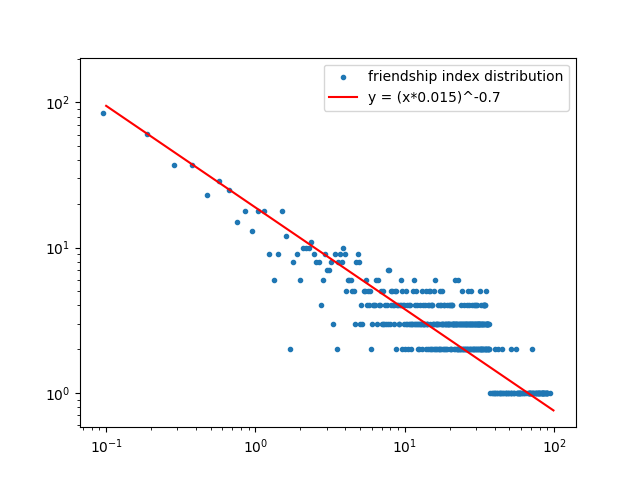
\includegraphics[scale=0.5]{C:/Users/YURA/source/repos/CSW/diploma_results/static_log/ba_dist_beta_5.png}
 \caption{Distribution of the friendship index in the \\Barabasi"---Albert model \\with $m=5$}
\end{figure}
\begin{figure}[!ht]
    \centering
    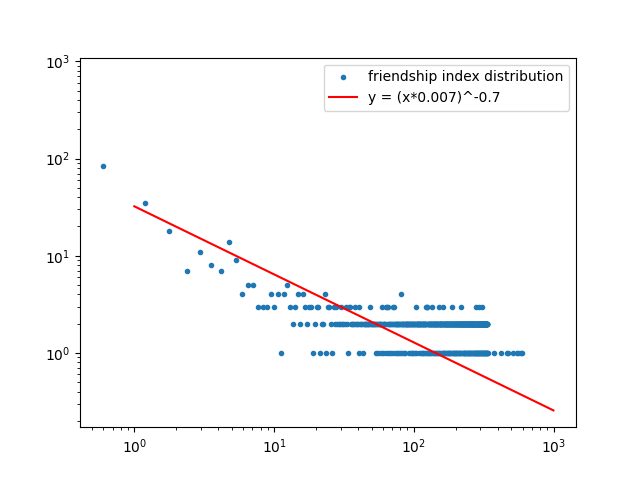
\includegraphics[scale=0.5]{C:/Users/YURA/source/repos/CSW/diploma_results/static_log/bap_dist_beta_4.png}
 \caption{Distribution of the friendship index in the \\Barabasi"---Albert model \\with a Poisson distribution\\of degrees of new vertices \\for $ \lambda=4$}
\end{figure}
\begin{figure}[!ht]
    \centering
    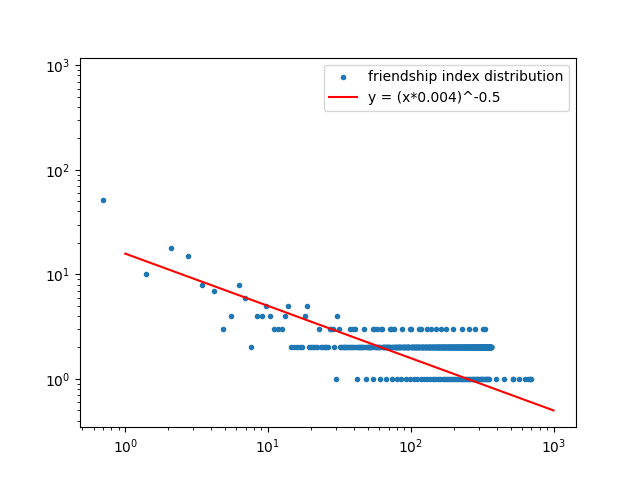
\includegraphics[scale=0.5]{C:/Users/YURA/source/repos/CSW/diploma_results/static_log/bap_dist_beta_5.png}
 \caption{Distribution of the friendship index in the \\Barabasi"---Albert model \\with a Poisson distribution\\of degrees of new vertices \\for $ \lambda=5$}
\end{figure}
\begin{figure}[!ht]
    \centering
    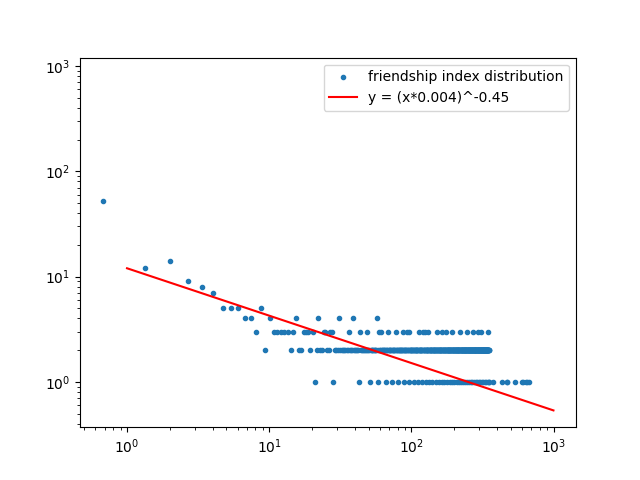
\includegraphics[scale=0.5]{C:/Users/YURA/source/repos/CSW/diploma_results/static_log/bap_dist_beta_6.png}
 \caption{Distribution of the friendship index in the \\Barabasi"---Albert model \\with a Poisson distribution\\of degrees of new vertices \\for $ \lambda=6$}
\end{figure}
\begin{figure}[!ht]
    \centering
    \includegraphics[scale=0.5]{C:/Users/YURA/source/repos/CSW/diploma_results/static_log/triad_dist_beta_3_0.25.png}
 \caption{Friendship index distribution in\\triad closure model\\with $m=3$ and $p=0.25$}
\end{figure}
\begin{figure}[!ht]
    \centering
    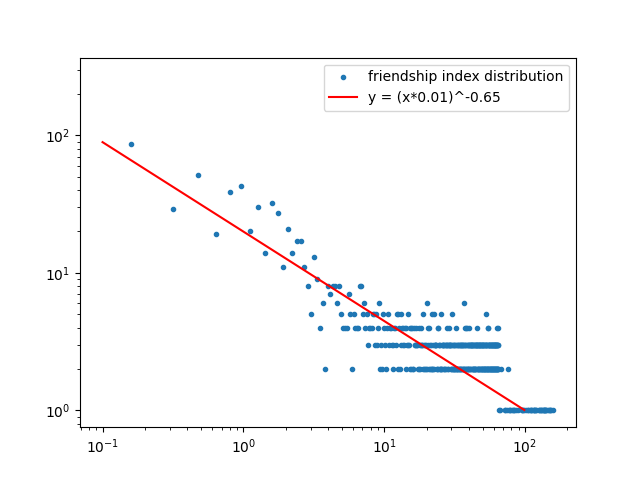
\includegraphics[scale=0.5]{C:/Users/YURA/source/repos/CSW/diploma_results/static_log/triad_dist_beta_3_0.5.png}
 \caption{Friendship index distribution in\\triad closure model\\with $m=3$ and $p=0.5$}
\end{figure}
\begin{figure}[!ht]
    \centering
    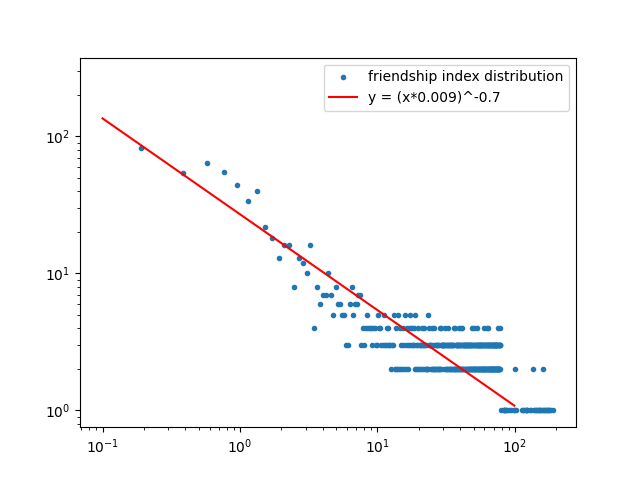
\includegraphics[scale=0.5]{C:/Users/YURA/source/repos/CSW/diploma_results/static_log/triad_dist_beta_3_0.75.png}
 \caption{Friendship index distribution in \\triad closure model\\with $m=3$ and $p=0.75$}
\end{figure}
\begin{figure}[!ht]
    \centering
    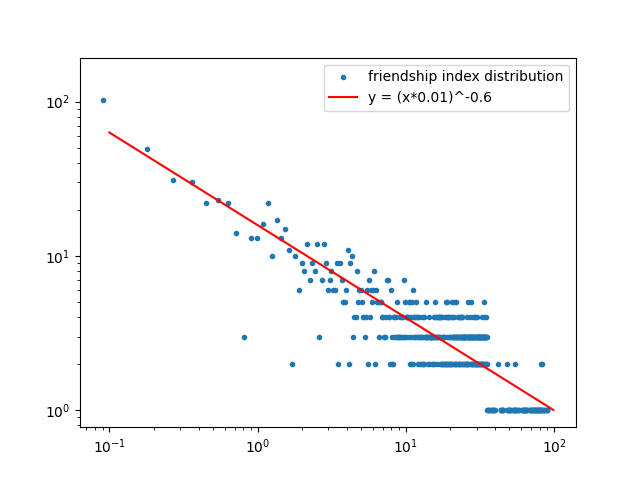
\includegraphics[scale=0.5]{C:/Users/YURA/source/repos/CSW/diploma_results/static_log/triad_dist_beta_5_0.25.png}
 \caption{Friendship index distribution in\\triad closure model\\with $m=5$ and $p=0.25$}
\end{figure}
\begin{figure}[!ht]
    \centering
    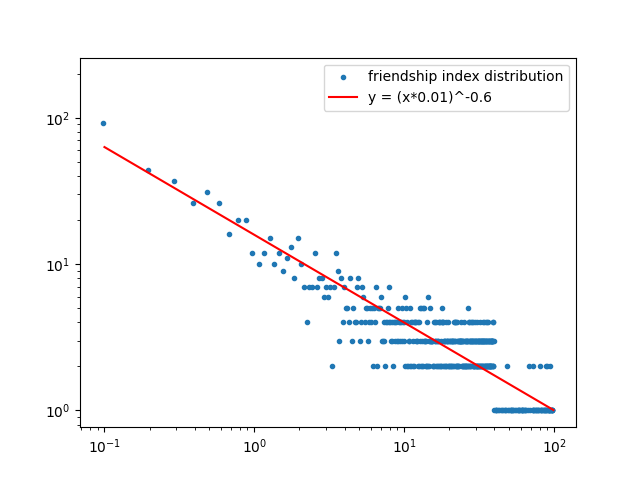
\includegraphics[scale=0.5]{C:/Users/YURA/source/repos/CSW/diploma_results/static_log/triad_dist_beta_5_0.5.png}
 \caption{Friendship index distribution in\\triad closure model\\with $m=5$ and $p=0.5$}
\end{figure}
\begin{figure}[!ht]
    \centering
    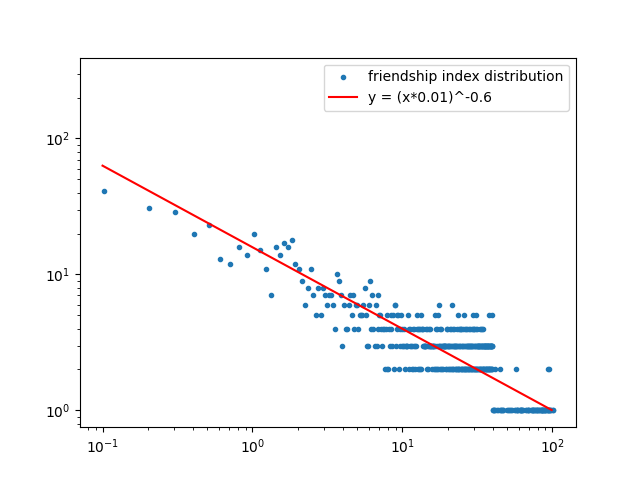
\includegraphics[scale=0.7]{C:/Users/YURA/source/repos/CSW/diploma_results/static_log/triad_dist_beta_5_0.75.png}
 \caption{Friendship index distribution in \\triad closure model\\with $m=5$ and $p=0.75$}
\end{figure}
\section{Plots of the dynamics of the average friendship index in the constructed graphs}\label{app:dyn}
\begin{figure}[!ht]
    \centering
    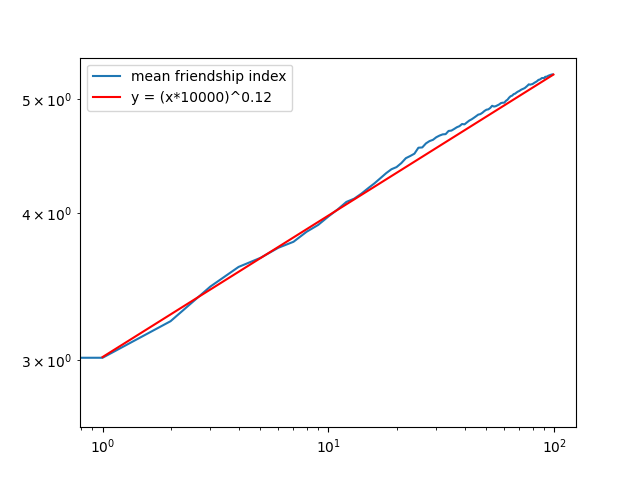
\includegraphics[scale=0.7]{C:/Users/YURA/source/repos/CSW/diploma_results/dynamic_log/ba_mean_beta_3.png}
 \caption{Dynamics of the average friendship index in the \\Barabasi"---Albert model \\with $m=3$}
\end{figure}
\begin{figure}[!ht]
    \centering
    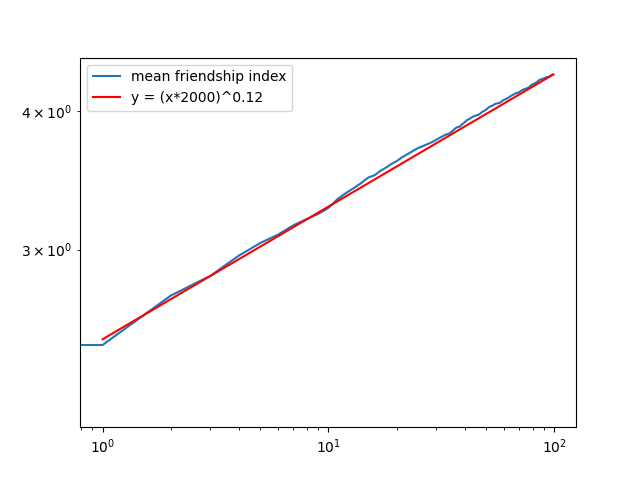
\includegraphics[scale=0.7]{C:/Users/YURA/source/repos/CSW/diploma_results/dynamic_log/ba_mean_beta_5.png}
 \caption{Dynamics of the average friendship index in the \\Barabasi"---Albert model \\with $m=5$}
\end{figure}
\begin{figure}[!ht]
    \centering
    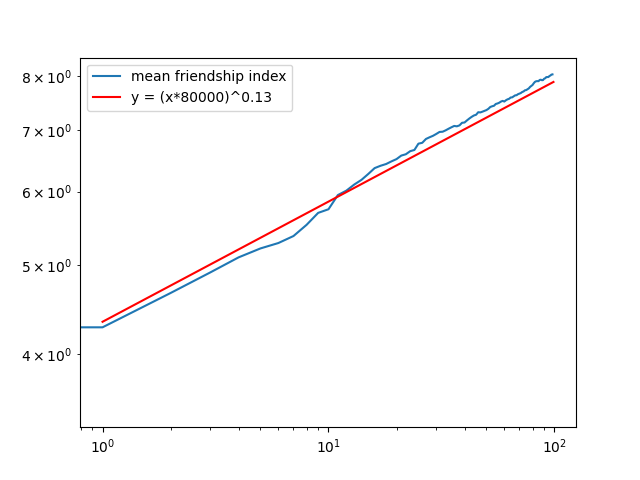
\includegraphics[scale=0.7]{C:/Users/YURA/source/repos/CSW/diploma_results/dynamic_log/bap_mean_beta_4.png}
 \caption{Dynamics of the average friendship index in the \\Barabasi"---Albert model \\with Poisson distribution\\degrees of new vertices \\with $ \lambda=4$}
\end{figure}
\begin{figure}[!ht]
    \centering
    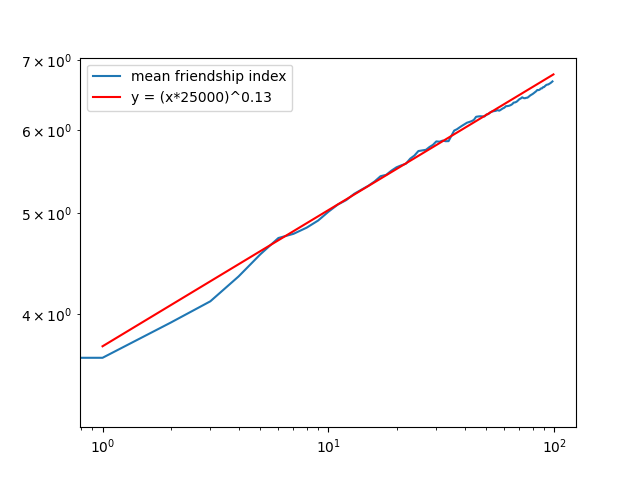
\includegraphics[scale=0.7]{C:/Users/YURA/source/repos/CSW/diploma_results/dynamic_log/bap_mean_beta_5.png}
 \caption{Dynamics of the average friendship index in the \\Barabasi"---Albert model \\with Poisson distribution\\degrees of new vertices \\with $ \lambda=5$}
\end{figure}
\begin{figure}[!ht]
    \centering
    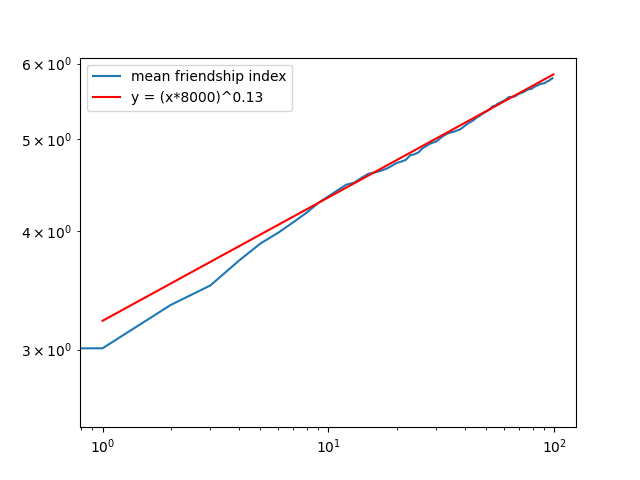
\includegraphics[scale=0.7]{C:/Users/YURA/source/repos/CSW/diploma_results/dynamic_log/bap_mean_beta_6.png}
 \caption{Dynamics of the average friendship index in the \\Barabasi"---Albert model \\with Poisson distribution\\degrees of new vertices \\with $ \lambda=6$}
\end{figure}
\begin{figure}[!ht]
    \centering
    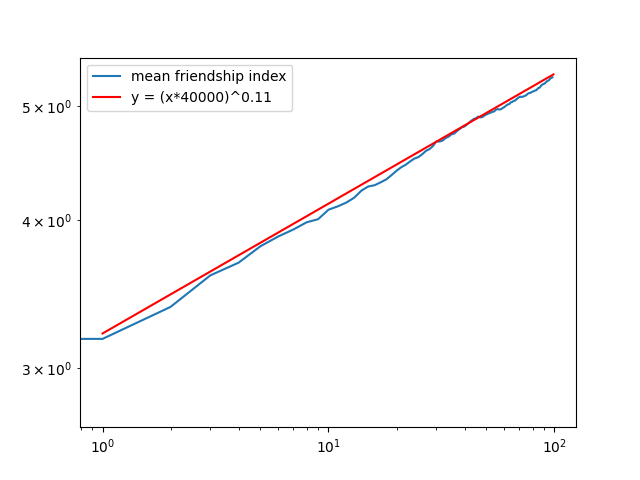
\includegraphics[scale=0.7]{C:/Users/YURA/source/repos/CSW/diploma_results/dynamic_log/triad_mean_beta_3_0.25.png}
 \caption{Dynamics of the average friendship index in the\\triad closure model\\with $m=3$ and $p=0.25$}
\end{figure}
\begin{figure}[!ht]
    \centering
    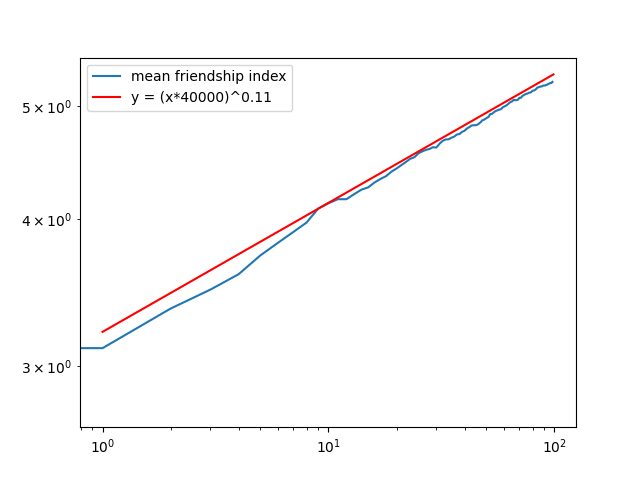
\includegraphics[scale=0.7]{C:/Users/YURA/source/repos/CSW/diploma_results/dynamic_log/triad_mean_beta_3_0.5.png}
 \caption{Dynamics of the average friendship index in the\\triad closure model\\with $m=3$ and $p=0.5$}
\end{figure}
\begin{figure}[!ht]
    \centering
    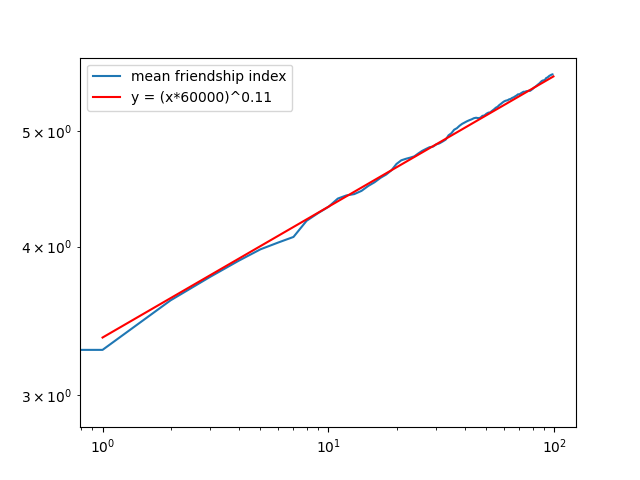
\includegraphics[scale=0.7]{C:/Users/YURA/source/repos/CSW/diploma_results/dynamic_log/triad_mean_beta_3_0.75.png}
 \caption{Dynamics of the average friendship index in the\\triad closure model\\with $m=3$ and $p=0.75$}
\end{figure}
\begin{figure}[!ht]
    \centering
    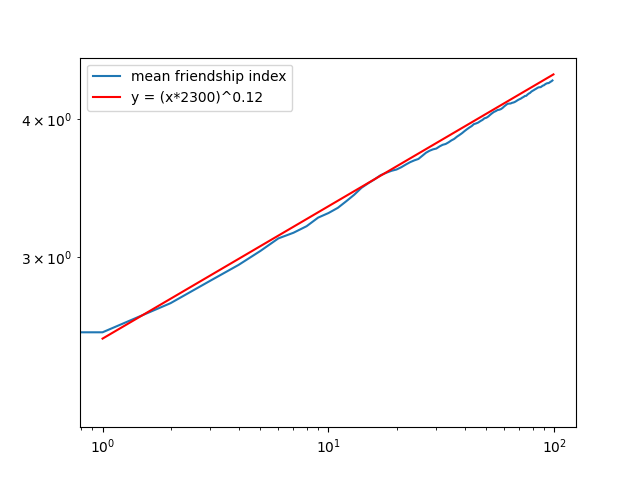
\includegraphics[scale=0.7]{C:/Users/YURA/source/repos/CSW/diploma_results/dynamic_log/triad_mean_beta_5_0.25.png}
 \caption{Dynamics of the average friendship index in the\\triad closure model\\with $m=5$ and $p=0.25$}
\end{figure}
\begin{figure}[!ht]
    \centering
    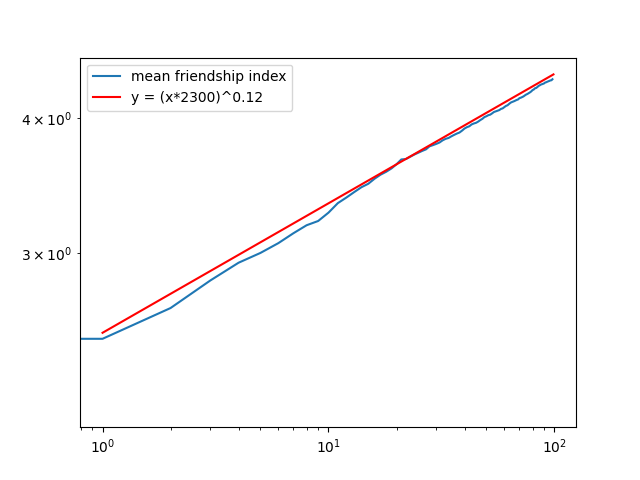
\includegraphics[scale=0.7]{C:/Users/YURA/source/repos/CSW/diploma_results/dynamic_log/triad_mean_beta_5_0.5.png}
 \caption{Dynamics of the average friendship index in the\\triad closure model\\with $m=5$ and $p=0.5$}
\end{figure}
\begin{figure}[!ht]
    \centering
    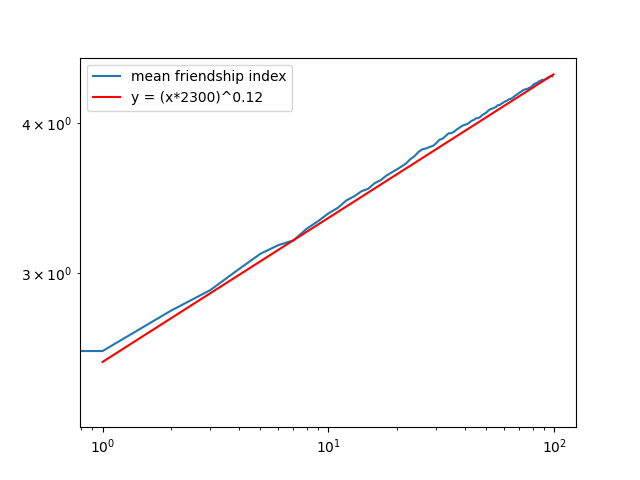
\includegraphics[scale=0.7]{C:/Users/YURA/source/repos/CSW/diploma_results/dynamic_log/triad_mean_beta_5_0.75.png}
 \caption{Dynamics of the average friendship index in the\\triad closure model\\with $m=5$ and $p=0.75$}
\end{figure}
\section{Script text for displaying the friendship index distribution}\label{app:rgs}
\begin{minted}{python}
import igraph
import numpy as np
import matplotlib.pyplot as plt
import os
import multiprocessing 
import math
def static(name):
    file = open('\\source\\repos\\CSW\\real_graphs\\' + name + '.txt', 'r')
    res = []
    degrees = {}
    while True:
        line = file.readline()
        if not line:
            break
        edge = [int(j) for j in line.split(" ")]
        if not edge[0] in degrees:
            degrees[edge[0]] = 0
        degrees[edge[0]] += 1
        if not edge[1] in degrees:
            degrees[edge[1]] = 0
        degrees[edge[1]] += 1
    file.seek(0)
    sums = {}
    while True:
        line = file.readline()
        if not line:
            break
        edge = [int(j) for j in line.split(" ")]
        if not edge[0] in sums:
            sums[edge[0]] = 0
        sums[edge[0]] += degrees[edge[1]]
        if not edge[1] in sums:
            sums[edge[1]] = 0
        sums[edge[1]] += degrees[edge[0]]
    for i in degrees.keys():
        res.append(sums[i] / degrees[i] / degrees[i])
    file.close()
    bincnt = 100000
    ans = np.histogram(res, bincnt)
    x = ans[1]
    y = ans[0]
    x = np.resize(x, x.size - 1)
    plt.bar(x[0:int(bincnt / 100 * 2)], y[0:int(bincnt / 100 * 2)])
    plt.show()
    plt.clf()
if __name__ == "__main__":
    static('sx-askubuntu')
\end{minted}
\section{Script text for displaying the dynamics of the friendship index}\label{app:rg}
\begin{minted}{python}
import igraph
import numpy as np
import matplotlib.pyplot as plt
import os
import multiprocessing 
import math
import datetime
def dynamics(name):
    file = open('\\source\\repos\\CSW\\real_graphs\\' + name, 'r')
    edge_list = []
    while True:
        line = file.readline()
        edge_list.append(line.split("\t"))
        if not line:
            break
    edge_list.pop()
    edge_list = [[i[0], 
                  i[1], 
                  datetime.datetime.strptime(i[3], '%Y-%m-%d %H:%M:%S').timestamp()] 
                 for i in edge_list]
    file.close()
    edge_list.sort(key = lambda i: i[2])
    step = 1000
    base = edge_list[0][2]
    res = []
    degrees = {}
    neibours_degrees = {}
    neibours = {}
    cnt = 0
    for i in edge_list:
        cnt += 1
        if not i[0] in degrees:
            degrees[i[0]] = 0
            neibours[i[0]] = set()
            neibours_degrees[i[0]] = 0
        if not i[1] in degrees:
            degrees[i[1]] = 0
            neibours[i[1]] = set()
            neibours_degrees[i[1]] = 0
        if i[0] == i[1]:
            degrees[i[0]] += 1
            neibours_degrees[i[0]] += degrees[i[0]]
            for j in neibours[i[0]]:
                neibours_degrees[j] += 1
            neibours[i[0]].add(i[0])
        else:
            degrees[i[0]] += 1
            degrees[i[1]] += 1
            if not i[1] in neibours[i[0]] and not i[0] in neibours[i[1]]:
                neibours_degrees[i[0]] += degrees[i[1]]
                neibours_degrees[i[1]] += degrees[i[0]]
            for j in neibours[i[0]]:
                neibours_degrees[j] += 1
            for j in neibours[i[1]]:
                neibours_degrees[j] += 1
            neibours[i[0]].add(i[1])
            neibours[i[1]].add(i[0])
        if (i[2] - base) >= step:
            base = step * math.ceil(i[2] / step)
            ans = []
            for j in degrees.keys():
                ans.append(neibours_degrees[j] / degrees[j] / degrees[j])
            res.append(np.mean(ans))
        # if cnt % step == 0:
        #     ans = []
        #     for j in degrees.keys():
        #         ans.append(neibours_degrees[j] / degrees[j] / degrees[j])
        #     res.append(np.mean(ans))
    plt.plot(res)
    plt.savefig("\\source\\repos\\CSW\\diploma_results\\" + name + "_iterational_dynamics.jpg")
    plt.clf()  
def run_thread(namegroup, i, res):
    ans = []
    for j in namegroup:
        ans.append(dynamics(j))
    res[i] = ans
def run(names):
    procs = []
    manager = multiprocessing.Manager()
    res = manager.dict()
    for (i, namegroup) in enumerate(names):
        p = multiprocessing.Process(target=run_thread, args=(namegroup, i, res))
        procs.append(p)
        p.start()
    for proc in procs:
        proc.join()
    ans = []
    for i in res.values():
        ans += i
    return ans
if __name__ == "__main__":
    # run([['askubuntu', 'askubuntu-a2q'], ['askubuntu-c2a', 'askubuntu-c2q'], ['mathoverflow', 'mathoverflow-a2q'], 
    #      ['mathoverflow-c2a', 'mathoverflow-c2q'], ['superuser', 'superuser-a2q'], ['superuser-c2a', 'superuser-c2q']])
    dynamics('soc-redditHyperlinks-body.tsv')
\end{minted}
\section{Script text for displaying the dynamics of the friendship index in graphs presented in several files}\label{app:rgp}
\begin{minted}{python}
import igraph
import numpy as np
import matplotlib.pyplot as plt
import os
import multiprocessing 
import math
import datetime
def dynamics(name):
    file = open('\\source\\repos\\CSW\\real_graphs\\' + name + '.txt', 'r')
    time_file = open('\\source\\repos\\CSW\\real_graphs\\' + name + '-dates.txt', 'r')
    times = {}
    while True:
        line = time_file.readline()
        if not line:
            break
        line = line.split("\t")
        line = [int(line[0]), int(line[1].replace('-', ''))]
        times[line[0]] = line[1]
    edge_list = []
    while True:
        line = file.readline()
        edge_list.append(line.split("\t"))
        if not line:
            break
    edge_list.pop()
    edge_list = [[int(j) for j in i] for i in edge_list]
    file.close()
    time_file.close()
    edge_list.sort(key = lambda i: times[i[0]] if i[0] in times else 100000000)
    step = 1000
    # base = edge_list[0][2]
    res = []
    degrees = {}
    neibours_degrees = {}
    neibours = {}
    cnt = 0
    for i in edge_list:
        cnt += 1
        if not i[0] in degrees:
            degrees[i[0]] = 0
            neibours[i[0]] = set()
            neibours_degrees[i[0]] = 0
        if not i[1] in degrees:
            degrees[i[1]] = 0
            neibours[i[1]] = set()
            neibours_degrees[i[1]] = 0
        if i[0] == i[1]:
            degrees[i[0]] += 1
            neibours_degrees[i[0]] += degrees[i[0]]
            for j in neibours[i[0]]:
                neibours_degrees[j] += 1
            neibours[i[0]].add(i[0])
        else:
            degrees[i[0]] += 1
            degrees[i[1]] += 1
            if not i[1] in neibours[i[0]] and not i[0] in neibours[i[1]]:
                neibours_degrees[i[0]] += degrees[i[1]]
                neibours_degrees[i[1]] += degrees[i[0]]
            for j in neibours[i[0]]:
                neibours_degrees[j] += 1
            for j in neibours[i[1]]:
                neibours_degrees[j] += 1
            neibours[i[0]].add(i[1])
            neibours[i[1]].add(i[0])
        # if (i[2] - base) >= step:
        #     base = step * math.ceil(i[2] / step)
        #     ans = []
        #     for j in degrees.keys():
        #         ans.append(neibours_degrees[j] / degrees[j] / degrees[j])
        #     res.append(np.mean(ans))
        if cnt % step == 0:
            ans = []
            for j in degrees.keys():
                ans.append(neibours_degrees[j] / degrees[j] / degrees[j])
            res.append(np.mean(ans))
    plt.plot(res)
    plt.savefig("\\source\\repos\\CSW\\diploma_results\\" + name + "_iterational_dynamics.jpg")
    plt.clf()
if __name__ == "__main__":
    # run([['askubuntu', 'askubuntu-a2q'], ['askubuntu-c2a', 'askubuntu-c2q'], ['mathoverflow', 'mathoverflow-a2q'], 
    #      ['mathoverflow-c2a', 'mathoverflow-c2q'], ['superuser', 'superuser-a2q'], ['superuser-c2a', 'superuser-c2q']])
    dynamics('cit-Patents')
\end{minted}

\section{Graphs of the distribution and dynamics of the friendship index in real networks}\label{app:real}
\begin{figure}[!ht]
    \centering
    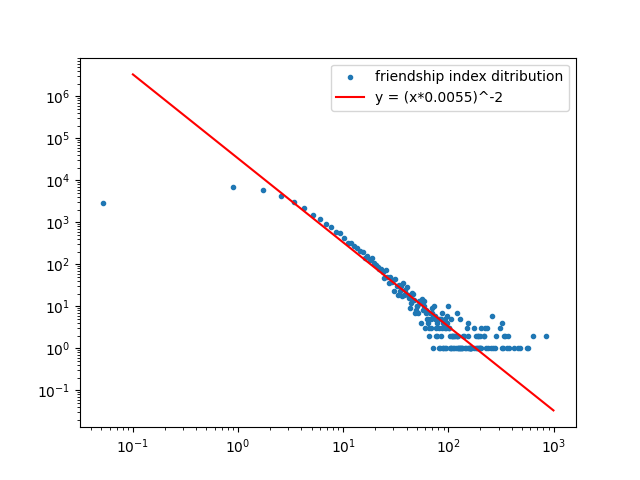
\includegraphics[scale=0.5]{C:/Users/YURA/source/repos/CSW/diploma_results/static_real_log/Cit-HepPh.png}
 \caption{Distribution of the friendship index in the \\citation network of articles in the field of \\high energy physics phenomenology\\on the logarithmic scale}
\end{figure}
\begin{figure}[!ht]
    \centering
    \includegraphics[scale=0.5]{C:/Users/YURA/source/repos/CSW/diploma_results/dynamic_real_log/Cit-HepPh_mean.png}
 \caption{Dynamics of the friendship index in the \\network of citations of articles in the field of \\phenomenology of high energy physics\\on the logarithmic scale}
\end{figure}
\begin{figure}[!ht]
    \centering
    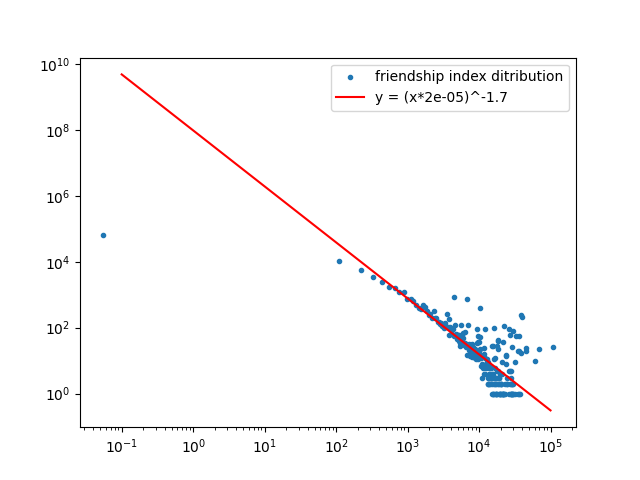
\includegraphics[scale=0.5]{C:/Users/YURA/source/repos/CSW/diploma_results/static_real_log/gplus_combined.png}
 \caption{Distribution of the friendship index in\\Google+ social network\\on the logarithmic scale}
\end{figure}
\begin{figure}[!ht]
    \centering
    \includegraphics[scale=0.5]{C:/Users/YURA/source/repos/CSW/diploma_results/dynamic_real_log/CollegeMsg_mean.png}
 \caption{Dynamics of the friendship index in the\\message network of students at the University of California, Irvine\\on the logarithmic scale}
\end{figure}
\begin{figure}[!ht]
    \centering
    \includegraphics[scale=0.5]{C:/Users/YURA/source/repos/CSW/diploma_results/static_real_log/CollegeMsg.png}
 \caption{Distribution of the friendship index in the\\UC Irvine student message network\\on the logarithmic scale}
\end{figure}

\end{document}